\chapter{Parallel method for generating pairs}
\label{chap:pairs}

A congruence is a binary relation, and therefore is formally described as a set
of pairs.  In a computational setting, it is rarely practical to keep track of
every pair in a congruence; a congruence on a semigroup of size $n$ contains
$n^2$ pairs in the worst case, and on an infinite semigroup contains an infinite
number of pairs.  A congruence can be described in more concise ways:
for example, taking advantage of it being an equivalence relation
and recording only its equivalence classes; or in the case of a Rees congruence,
storing a generating set for the ideal which defines it.  A variety of different
ways to describe a congruence are explained in Chapter \ref{chap:converting},
along with ways to convert from one to another.  However, a congruence is still just
a set of pairs, and by reducing the number of pairs we store, we can often describe a
congruence very concisely using them.

\begin{definition}
  Let $S$ be a semigroup and let $R$ be a subset of $S \times S$.
  \begin{itemize}
  \item
    The \textbf{congruence generated by} $R$ is the least congruence
    (with respect to containment) that contains $R$ as a subset.
  \item
    The \textbf{left congruence generated by} $R$ is the least left congruence
    (with respect to containment) that contains $R$ as a subset.
  \item
    The \textbf{right congruence generated by} $R$ is the least right congruence
    (with respect to containment) that contains $R$ as a subset.
  \end{itemize}
\end{definition}

This definition is based on a simple intuitive idea:
a congruence $\rho$ is generated by a set of pairs $R$ if it consists
of only the pairs in $R$ along with the pairs required by the axioms of a
congruence (reflexivity, symmetry, transitivity and compatibility).  Thus a
congruence can be described completely by storing only a few pairs.
Indeed, experiments on a range of interesting semigroups in Chapter
\ref{chap:lattice} show that many congruences can be generated by an extremely
small number of generating pairs, and indeed that most of the congruences
studied are principal (generated by a single pair). %TODO: actually do this

Another justification for the use of generating pairs is that it is a completely
generic representation.  Some special types of semigroup have their own abstract
representations of congruences---for inverse semigroups, one can study
kernel-trace pairs \cite[\S 5.3]{howie}; for groups, normal subgroups
\cite[Theorem 11.5]{warner}; for completely simple or completely 0-simple
semigroups, linked triples \cite[\S 3.5]{howie}---but generating pairs can
represent a congruence on any semigroup whatsoever.  Furthermore, one
might be interested in what pairs are implied by a given pair or set of pairs in
a congruence, and this representation can answer such questions.

Left congruences and right congruences can also be described using generating
pairs, and some algorithms designed for two-sided congruences can be used with
minor modifications to compute information about left and right congruences.

This chapter describes a parallelised approach for computing a congruence from a
set of generating pairs, as implemented in \texttt{libsemigroups}
\cite{libsemigroups}.  First we will give a general outline of the system
and what questions it hopes to answer, then we will describe in detail each
algorithm used, its advantages and disadvantages, and when it can be applied.
Finally we will explain how the different algorithms are executed together, and
consider their implementation in \cite{libsemigroups}.

\section{Reasons for parallelisation}

Parallel processing has seen major advances in the last ten years, with
multi-core processors becoming the norm in many types of computers, and
processors with 4, 8, or even 16 cores becoming common on a desktop PC.  This
being the case, it is desirable to parallelise mathematical algorithms wherever
possible, and take advantage of the ability to execute multiple
threads of instructions concurrently.  Some algorithms
are ``embarrassingly parallel''---that is, they can be split into
independent threads which require almost no communication with each other.
Examples of these algorithms would be brute force searches, or rendering of
computer graphics.
These are suited so well to parallelisation that splitting the operation into
$n$ parallel threads reduces the expected run-time to barely more than
$\frac{1}{n}$ what it would be when run in a single thread.  Other
% TODO: don't say "1/n what it would be"
algorithms do not parallelise so well: sometimes threads have to communicate, or
use shared resources, causing significant slowdown and severely limiting the
improvements that can be made by parallelising.

When it comes to computing information about a congruence from generating pairs,
there are various different approaches which can be taken: in Sections
\ref{sec:p}, \ref{sec:tc} and \ref{sec:kb}, we describe three possible
algorithms: pair orbit enumeration, Todd-Coxeter, and Knuth-Bendix/Froidure-Pin.
Depending on what sort of semigroup is given as an input (see Section
\ref{sec:program-outputs}), several
or all of these might be appropriate.  However, depending on certain properties
of the congruence, one might perform far better than another.  For example, the
pair orbit algorithm works well on congruences that contain few non-reflexive
pairs, while the Todd-Coxeter algorithm tends to work well on congruences with
few classes (i.e.~very many pairs).  For a detailed analysis of which algorithms
perform well on which inputs, see Section \ref{sec:benchmarking}.  Given
only a set of generating pairs, these properties are likely to be unknown in
advance, which makes it difficult to choose a good algorithm.

The natural answer to this problem is the core concept of this chapter: a
parallel approach which does not attempt to parallelise individual algorithms,
but which runs several known algorithms at the same time, each in a different
thread, and simply halts all threads as soon as any one completes.  Since these
algorithms do not interact with each other in any way, the total run-time will
be close to the minimum run-time of all the different algorithms.  This is
particularly important, since for certain semigroups and congruences some
algorithms will never terminate, while others may terminate in a very short
time.

\section{Applicable types of semigroup}
\label{sec:applicable-types-of-semigroup}

The type of element in a semigroup affects which methods will be most effective,
or even which methods will be applicable.  For this purpose, we divide
semigroups into two categories: finitely presented semigroups, and
\textit{concrete} semigroups.

\begin{definition}
  \label{def:concrete}
  A semigroup $S$ is \textbf{concrete} if it is finite, and lies in a category
  with decidable word problem; that is, for a generating set $X$ for $S$, and
  any two words $w_1$ and $w_2$ in $X^+$, it can always be decided in a finite
  time whether $w_1$ and $w_2$ represent the same element of $S$.
\end{definition}

Concrete semigroups can have many different forms.  Perhaps the most trivial and
obvious example of a concrete semigroup would be a semigroup specified by a
Cayley table: the generating set $X$ contains all the elements of $S$, and two
words $w_1$ and $w_2$ represent the same element if and only if they produce the
same number when processed through the Cayley table.  Semigroups specified by
Cayley tables are therefore concrete; but in practice they are used very little,
since they require a great deal of space to store---order $O(|S|^2)$.

A more common representation is a transformation semigroup, or a semigroup of
partial permutations.  These contain elements which can be multiplied and
compared without reference to the semigroup as a whole: for example, if
$x = \transV 13342$ and $y = \transV 24422$ then we can calculate
$xy = \transV 24424$ without knowing anything about $S$, the semigroup that
contains $x$ and $y$.  So long as all elements in these semigroups have finite
degree, any multiplication or comparison is guaranteed to complete in a finite
time, and so the word problem on such a semigroup $S$ is decidable, and $S$ is
concrete.

Finitely presented semigroups are a different case, in that their elements
cannot be compared without reference to the semigroup as a whole.  If $S$ is a
semigroup described by a finite presentation $\pres X R$, and $w_1$ and $w_2$
are words in $X^+$, then it may be undecidable whether $w_1$ and $w_2$ represent
the same element of $S$.  There are many examples of presentations for which
this word problem is undecidable (see Example \ref{ex:makanin}), and so
semigroups specified by finite presentations are not concrete.  Besides, many
finite presentations describe infinite semigroups, and the finiteness of $S$ is
also not known in advance.

Decidability is discussed further in Section \ref{sec:decidability}.

Finitely presented monoids are treated as equivalent to finitely presented
semigroups, since a semigroup presentation can be attained by simply adding a
generator for the identity and relations to make it multiplicatively neutral.

\section{Program inputs}
\label{sec:program-inputs}

Our algorithm determines the properties of a single left, right, or two-sided
congruence defined by generating pairs, over a semigroup $S$.
For the remainder of this chapter, the word ``congruence'' will be used to refer
to left, right, and two-sided congruences equally, without having the default
meaning of ``two-sided congruence''. % TODO: move this warning?

If $S$ is a concrete semigroup (as described in Section
\ref{sec:applicable-types-of-semigroup}) then it will almost certainly be
specified by a generating set; in this case, it is quick to use these generators
to calculate a list of elements in $S$, along with left and right Cayley graphs
for $S$, using the Froidure-Pin algorithm (see Section \ref{sec:find-pres}).  If on the
other hand $S$ is a finitely presented semigroup, then the elements will not be
known in advance.  In either case, a finite presentation $\pres X R$ can be
given---a technique for efficiently finding a presentation for a concrete
semigroup is given in Section \ref{sec:find-pres}.
The exact parameters supplied to the algorithm are therefore as follows:
\begin{itemize}
\item A set of generators $X$;
\item A finite set of relations $R \subseteq X^* \times X^*$;
\item A finite set of generating pairs $W \subseteq X^* \times X^*$;
\item A record of whether we are computing a left, right, or two-sided
  congruence.
\end{itemize}
The following are also supplied if and only if $S$ is concrete:
\begin{itemize}
\item A list of elements of $S$;
\item Left and right Cayley graphs for $S$ (see Definition
  \ref{def:cayley-graph});
\item A factorisation function $f : S \to X^*$.
\end{itemize}

We shall now make clear the meanings of these different parameters, by giving a
complete description of the system, starting with the commutative diagram in
Figure \ref{fig:pairs-cd-1}.

Here $X$ is our alphabet, a subset of the free semigroup $X^+$.  We have a set
of relations $R \subseteq X^+ \times X^+$, which generates the congruence
$R^\sharp$ on $X^+$.  This congruence gives a quotient semigroup
$X^+ / R^\sharp$; this is isomorphic to the semigroup $S$,
which is described by the presentation $\pres X R$.  The
congruence also gives us its natural homomorphism $\pi: X^+ \to S$ (see
Definition \ref{def:natural-homomorphism}).  We also have a set of generating pairs
$\mathbf{P} \subseteq S \times S$, which defines a congruence
$\mathbf{P}^\sharp$.  The aim of the algorithm described in this chapter is to
obtain a data structure for $\mathbf{P}^\sharp$, where the precise meaning of
``data structure'' is defined in Section \ref{sec:program-outputs}.  If we are
calculating a two-sided congruence, then it gives rise to the
quotient semigroup $S / \mathbf{P}^\sharp$.

\begin{figure}[h]
  \centering
  $\begin{tikzcd}
    X \arrow[dr] \arrow[d, hook] & \\
    X^+ \arrow[r, two heads, "\pi"] & \frac{X^+}{R^\sharp} \cong S \arrow[r, two heads] & \frac{S}{\mathbf{P}^\sharp}
  \end{tikzcd}$
  \caption{The relationships between different input objects}
  \label{fig:pairs-cd-1}
\end{figure}

The generating pairs $\mathbf{P}$ are not given by the user.  Since the elements
of $S$ might be unknown (for example if $S$ was specified by a finite
presentation), it would be impractical for the user to specify them precisely.
Instead, the user specifies a set $W$ consisting of pairs of words from
$X^+ \times X^+$, which can be evaluated to pairs of elements in $S \times S$,
giving the set of generating pairs $\mathbf{P}$.
More formally, let
$\Pi: X^+ \times X^+ \to S \times S$ be defined by
$\Pi: (w_1, w_2) \mapsto (w_1\pi, w_2\pi)$, where $\pi$ is the natural
homomorphism from $X^+$ to $S$ mentioned above.  The generating pairs
$\mathbf{P}$ of the congruence are given by $\mathbf{P} = W \Pi$.
This relationship is summarised in Figure \ref{fig:pairs-cd-2}.

\begin{figure}[h]
  \centering
  $\begin{tikzcd}
    W \arrow[r, hook, two heads, "\Pi|_W"] \arrow[d, hook] & \mathbf{P} \arrow[d, hook] \\
    X^+ \times X^+ \arrow[r, two heads, "\Pi"] & S \times S
  \end{tikzcd}$
  \caption{The generating pairs of the congruence}
  \label{fig:pairs-cd-2}
\end{figure}

\section{Program outputs}
\label{sec:program-outputs}

Each method we are about to explain can provide a variety of different pieces of
information, but it is important to consider which questions we aim to answer.
Our system should be able to return the following information about a given
congruence when requested:

\begin{itemize}
\item Presence of a given pair $(x,y)$ in the congruence
\item Number of congruence classes
\item The elements in each non-trivial congruence class
\item Class number of a given element
\end{itemize}

\section{Decidability}
\label{sec:decidability}

\begin{definition}
  \label{def:decidable}
  A problem is \textbf{decidable} if there exists an algorithm which is
  guaranteed to return a correct answer to the problem in a finite amount of
  time.
\end{definition}

Decidability is always something that should be considered when designing an
algorithm that may act on infinite objects.  In the context of this chapter, if
the semigroup $S$ is specified as a concrete semigroup, then all of the
questions defined in Section \ref{sec:program-outputs} have a definite answer
which can be calculated.  However, if $S$ is specified using a presentation,
then certain problems asked about it may be undecidable.

Firstly, we might consider the presence of a given pair $(x,y)$ in a given
congruence.  This is equivalent to solving the word problem for the quotient
semigroup of the congruence, and has long been known to be undecidable in
general.  Indeed, consider the following example from Gennadi\'{i} Makanin with
only three generators.

\begin{example}[Makanin, 1966]
  \label{ex:makanin}
  The presentation
  $$\pres{a,b,c}{c^2b^2 = b^2c^2,\ bc^3b^2 = cb^3c^2,\ ac^2b^2 = b^2a,\ abc^3b^2 = cb^2a,\ b^2c^2b^4c^2 = b^2c^2b^4c^2a}$$
  defines a semigroup which has undecidable word problem.  \cite{makanin_1966}
\end{example}
% TODO: read this properly, and maybe give a proof.

Furthermore, consider the following example from G.S.~Cijtin, perhaps the
simplest undecidable presentation, with 5 generators but only 33 occurrences of
those generators in its relations.

\begin{example}[Cijtin, 1957]
  \label{ex:cijtin}
  The presentation
  $$\pres{a,b,c,d,e}{ac=ca,\ ad=da,\ bc=cb,\ bd=db,\ ce=eca,\ de=edb,\ c^2e=c^2ae}$$
  defines a semigroup which has undecidable word problem.  \cite{cijtin_1957, collins_1986}
\end{example}
% TODO: read these properly, and maybe give proofs.

Since the general semigroup word problem is undecidable, the algorithm in this
chapter cannot hope to guarantee to return an answer.  Similarly, the number of
classes of a given congruence and the elements of each non-trivial class may not
be computable, since there may be infinitely many.

The only guarantee that can be given by the algorithm is that an answer will be
returned if $S$ happens to be finite.  In the concrete case, semigroups are
always finite and so an answer is guaranteed; but in the case of a finitely
presented semigroup, it is unknown in advance whether a semigroup is finite or
not.  Hence, the user of this algorithm might not know whether a particular run
is guaranteed to terminate, since a run that is about to finish is
indistinguishable from one that will run forever.

\section{Finding a presentation}
\label{sec:find-pres}

A concrete semigroup $S$ is not specified by a presentation, but by a set of
generators whose multiplication is well understood independent of $S$.  However,
a finite presentation is still required for the Todd-Coxeter and Knuth-Bendix
algorithms to be used, and so a presentation $\pres X R$ must be calculated for
a concrete semigroup.  For the purposes of the algorithm described in this
chapter, it is not important how this presentation is obtained, only that it is
correct and that elements from $S$ can be factorised with respect to $X$.

The \texttt{libsemigroups} implementation of this chapter's algorithm uses the
Froidure-Pin algorithm, a method which takes a concrete semigroup $S$ and a set
of generators $X$, and returns several useful pieces of information about it:
\begin{itemize}
\item a left Cayley graph for $S$ with respect to $X$;
\item a right Cayley graph for $S$ with respect to $X$;
\item a confluent terminating rewriting system $R$ describing the elements of
  $S$ as words in $X^+$;
\item and for each element $s \in S$, a word $w \in X^+$ representing one
  possible factorisation of $s$.
\end{itemize}
The right Cayley graph can be used by the Todd-Coxeter procedure to pre-fill its
table (see Section \ref{sec:tc-prefill}).  But more importantly, the rewriting
system $R$ is a set of pairs which can be used as the relations in a finite
presentation $\pres X R$ for the semigroup $S$.  The fact that $R$ is confluent
and terminating may also be useful when it is used as part of a rewriting system
in the Knuth-Bendix process later (see Section \ref{sec:kb}).

For more information about the Froidure-Pin algorithm and its implementation in
\texttt{libsemigroups}, see \cite{froidure-pin} and \cite{froidure-pin-jonusas}.

% TODO: actually describe it?

\section{The methods}

\subsection{Pair orbit enumeration}
\label{sec:p}

This is the simplest of the algorithms discussed in this section, and
generally does not perform as well as the others in practice.  However, it has certain
advantages such as its small overhead and quick setup, and therefore on certain (somewhat
trivial) examples performs better than the others.  Furthermore, it is
applicable to any problem discussed in this chapter, whether $S$ is a concrete
or finitely presented semigroup, and whether $\rho$ is a left, right or
two-sided congruence.

We will now give a brief description of pair orbit enumeration---a pseudo-code
description is shown in Algorithm \ref{alg:p}.  We start with a semigroup $S$, a
set of generators $X$ for $S$, and a set of generating pairs $\mathbf{R}$ for
the congruence we are trying to compute.  It will also be important to remember
whether we are calculating a left, right, or two-sided congruence, a piece of
information encoded in Algorithm \ref{alg:p} as $\sigma \in \{L,R,T\}$.  We
start with a list of pairs $\mathbf{R}'$ which we initialise to be equal
to the set of generating pairs $\mathbf{R}$; this list $\mathbf{R}'$ will hold
all the pairs that have been found so far, except those we infer from
reflexivity, symmetry and transitivity.  We also have a \textit{union-find}
table $\tau$, which will begin as an array of size $0$.  This table will be used
to keep track of which elements are in which class.  Union-find is a
well-established method for describing equivalence relations---see
\cite{union-find} for a more detailed description.

We now begin iterating through the pairs in $\mathbf{R}'$, and as we do so we
will add further pairs to $\mathbf{R}'$ which will also need to be iterated on,
until we reach the end of the list.  For each pair $(a,b)$ we first need to
merge $a$ and $b$ in the union-find table $\tau$---if either $a$ or $b$ does not
already have a position in $\tau$, then it will need to be added first.  Now,
for each generator $x$, we can find the two pairs $(xa,xb)$ and $(ax,ab)$.
Depending on whether we are calculating a left, right, or two-sided congruence,
we add one or both of these pairs to $\mathbf{R}'$ to be processed in its own
turn.

\begin{algorithm}
\caption{The pair orbit enumeration algorithm}
\label{alg:p}
\begin{algorithmic}[1]
\Require $S$ a semigroup,
         $\mathbf{R} \subseteq S \times S$,
         $\sigma \in \{L, R, T\}$
\Procedure{P}{$S, \mathbf{R}, \sigma$}
\State Let $X$ be a generating set for $S$
\State $\mathbf{R}' := \mathbf{R}$
%\Comment{$\mathbf{R}'$ is the list of pairs found so far}
\State $\tau :=$ an empty \textsc{Union-Find} table
\For{$(a,b) \in \mathbf{R}'$}
  \State \Call{Union}{$\tau, a, b$}
  \For{$x \in X$}
    \If{$\sigma \in \{L, T\}$}
      \State $\mathbf{R}' \gets \mathbf{R}' \cup \{(xa, xb)\}$
    \EndIf
    \If{$\sigma \in \{R, T\}$}
      \State $\mathbf{R}' \gets \mathbf{R}' \cup \{(ax, bx)\}$
    \EndIf
  \EndFor
\EndFor
\EndProcedure
\end{algorithmic}
\end{algorithm}

Once this procedure is finished, we have a complete table $\tau$ which describes
the congruence's non-trivial classes.  To check whether a pair $(a,b)$ lies in
the congruence, we now just need to look up $a$ and $b$ in the table using
\textsc{Find}, and if they lie in the same class we return true.  If either
element has not been added to $\tau$, then it lies in a singleton, and $(a,b)$
is only in the congruence if $a=b$.

It would be possible, instead of increasing the length of $\tau$ when a new
element is found, to make $\tau$'s original length equal to the size of $S$ at
creation.  However, this approach is not used here, since adding the elements only as
they are found opens up the possibility of applying this method to infinite
semigroups.  Our implementation in \texttt{libsemigroups} \cite{libsemigroups}
includes such a possibility, by taking a semigroup presentation $\pres X R$ and
using Knuth-Bendix (see Section \ref{sec:kb}) as a way of comparing the semigroup's
elements.  The pair orbit enumeration procedure, as described above, can then be
used, and will complete in finite time if and only if the number of elements in
non-trivial congruence classes is finite.  This was implemented to answer
questions other than checking a pair's inclusion in the congruence, and will
therefore not be discussed in any more detail in this chapter.

This algorithm's run-time is a product of the number of pairs in the congruence.
The algorithm is therefore quick to complete for congruences with few
non-reflexive pairs---that is, congruences with many classes.  Conversely, it is
exceedingly slow for congruences with many pairs and few classes.

Some improvements can be made to the basic algorithm shown above.  For example,
the \texttt{libsemigroups} implementation makes use of the symmetry of pairs: a
pair $(a,b)$ is not added to $\mathbf{R}'$ if the pair $(b,a)$ has previously
been added.  Tweaks like this can make the algorithm slightly faster, though
they do not address the high complexity of the method.

\subsection{Todd-Coxeter}
\label{sec:tc}

The Todd-Coxeter algorithm was originally described in 1936 in
\cite{todd_coxeter_1936}.  It was an algorithm to enumerate the cosets of a
finitely generated subgroup of a finitely presented group.  Arriving before the
advent of electronic computers, the algorithm was originally intended to be
carried out by hand.  Perhaps the earliest automatic implementation was on the
EDSAC II computer in Cambridge \cite{leech_1963}.  Since then, a wide variety of
efficient, optimised versions have been implemented, for example \cite{ace}.

A variation of Todd-Coxeter for semigroups was described in 1967
\cite{neumann_1967}.  The algorithm takes a presentation $\pres X R$
for a semigroup $S$ and computes the right regular representation of $S^1$ with
respect to the generators $X$---that is, it computes all the elements of $S$ and
the result of right-multiplying each element by each generator.  Since the
original algorithm makes very little use of those properties unique to groups,
the method applied to semigroups is essentially the same.  Other descriptions of
Todd-Coxeter for semigroups can be found in \cite[Chapter 12]{ruskuc_thesis} and
\cite[Chapter 1.2]{walker_thesis}, and a variation specific to inverse
semigroups can be found in \cite{cutting_thesis}.  Our version of the algorithm
is based closely on an implementation by G\"otz Pfeiffer, found in
\cite[\texttt{lib/tcsemi.gi}]{gap}, and based on \cite{walker_thesis}.

We will now describe the Todd-Coxeter method as used in the context of this
chapter.  Though the method itself does not represent new work, it is an
important part of the overall parallel approach, and in order to understand its
uses and limitations, it is described here in full.

\subsubsection{Setup}

The Todd-Coxeter algorithm is based on a table, where each row corresponds to a
single congruence class (or equivalently, a single element of the quotient
semigroup).  The columns of the table correspond to the generators of the
semigroup, and the entry in row $i$, column $j$ represents the element found by
taking element $i$ and right-multiplying it by generator $j$.  These entries may
be blank, and two different rows may be found to describe the same element.
Mathematically, we can view this table as a triple $(n, \mathbf{N}, \tau)$
consisting of:
\begin{itemize}
\item an integer $n \in \mathbb{N}$ representing the number of rows in the table;
\item a set $\mathbf{N} \subseteq \{1, \ldots, n\}$ containing the indices of the
  \textit{undeleted} rows; and
\item a function $\tau: \mathbf{N} \times X \to \mathbf{N} \cup \{0\}$, where
  $(i, x)\tau$ is equal to the entry in row $i$ and the column corresponding to
  generator $x$---with $0$ representing a blank entry.
\end{itemize}

Suppose that we have a semigroup presentation $\pres X R$ for a semigroup
$S$.  The table is initialised with a single row, numbered $1$.  This row
corresponds to the empty word $\varepsilon$, or the adjoined identity of the
monoid $S^1$.  The row is empty, containing a blank entry in all $|X|$ columns.
In our mathematical notation, we define $n=1$ and
$(1,x)\tau = 0$ for all $x \in X$.

We can naturally extend the function
$\tau: \mathbf{N} \times X \to \mathbf{N} \cup \{0\}$
to a function
$\bar{\tau}: \mathbf{N} \times X^* \to \mathbf{N} \cup \{0\}$
which is described as follows.
If $w \in X^*$ and $w=w_1 \ldots w_n$, where $w_1, \ldots, w_n \in X$,
then we can define $\bar\tau$ recursively by
$$
(i, w)\bar\tau = \left\{
\begin{matrix*}[l]
  i & \textnormal{if~} w=\varepsilon,\\
  0 & \textnormal{if~} (i, w_1)\tau=0,\\
  ((i, w_1)\tau, w_2 \ldots w_n)\bar\tau & \textnormal{otherwise}.
\end{matrix*} \right.
$$

The effect of $\bar\tau$ is to trace an entire word through the table, starting
at a given row.

\subsubsection{Elementary operations}

We now describe 3 operations which may be applied to the table.  These
operations will be described loosely to give an intuition behind what they are
designed to do, and then each one will be described formally in pseudo-code
(Algorithms \ref{alg:add}, \ref{alg:trace} and \ref{alg:coinc}).  We will then
describe the overall Todd-Coxeter procedure which uses these operations
(Algorithm \ref{alg:tc}).

\begin{itemize}
\item \textsc{Add}: Fill in a blank entry and add a row to the table;
\item \textsc{Trace}: Trace a relation from a row;
\item \textsc{Coinc}: Process a coincidence.
\end{itemize}

The first operation, \textsc{Add}, is simple.  A new row is added at the bottom
of the table, and its number is written into the blank cell in the table
specified by the arguments given to \textsc{Add}.  Pseudo-code for this
operation is given in Algorithm \ref{alg:add}.

\begin{algorithm}
\caption{The \textsc{Add} algorithm}
\label{alg:add}
\begin{algorithmic}[1]
\Procedure{Add}{$i, x$}
\State $n \gets n + 1$
\State $\mathbf{N} \gets \mathbf{N} \cup \{n\}$
\For{$x \in X$}
  \State $(n, x)\tau := 0$
\EndFor
\State $(i, x)\tau \gets n$
\EndProcedure
\end{algorithmic}
\end{algorithm}

\textsc{Trace} takes two arguments: a relation $v=w$ from $R$, and a row $e$
in the table.  We now give an informal description of this procedure---see
Algorithm \ref{alg:trace} for pseudo-code.

We start from row $e$, and find $(e, v)\bar\tau$ by processing $v$ one letter at a time: we
find the column corresponding to the letter, and look at that position in the
table; this gives us the number of the new row which we move to.  If we
encounter a blank entry before the final letter, we apply \textsc{Add} to that
cell, and follow the new entry.  At the end of the process we have an entry in
the table, blank or filled, called $(e, v)\bar\tau$.  We repeat the
process with the other word to find $(e, w)\bar\tau$.

To satisfy $v=w$, we need to set these two entries such that
$(e, v)\bar\tau = (e, w)\bar\tau$.
\begin{itemize}
\item If $(e, v)\bar\tau$ and $(e, w)\bar\tau$ are both blank, then we apply
  \textsc{Add} to $(e, v)\bar\tau$ and copy the entry into $(e, w)\bar\tau$.
\item If just one of the entries is filled, then the filled entry is copied into
  the blank one.
\item If both entries are filled and equal, we need do nothing.
\item If both entries are filled and are distinct, we apply \textsc{Coinc} to
  the two entries.
\end{itemize}

\begin{algorithm}
\caption{The \textsc{Trace} algorithm}
\label{alg:trace}
\begin{algorithmic}[1]
\Procedure{Trace}{$e, v = w$}
\State Write $v = v_1 \ldots v_m$ \Comment $(v_i \in X \text{~for~} 1 \leq i \leq m)$
\State Write $w = w_1 \ldots w_n$ \Comment $(w_i \in X \text{~for~} 1 \leq i \leq n)$
\State $s \gets e$
\For{$i \in \{1, \ldots, m-1\}$}
  \If{$(s, v_i)\tau = \varepsilon$}
    \State \Call{Add}{$s, v_i$}
  \EndIf
  \State $s \gets (s, v_i)\tau$
\EndFor
\State $t \gets e$
\For{$i \in \{1, \ldots, n-1\}$}
  \If{$(t, w_i)\tau = \varepsilon$}
    \State \Call{Add}{$t, w_i$}
  \EndIf
  \State $t \gets (t, w_i)\tau$
\EndFor

\If{$(s, v_m)\tau = (t, w_n)\tau = \varepsilon$}
  \State \Call{Add}{$s, v_m$}
  \State $(t, w_n)\tau \gets (s, v_m)\tau$
\ElsIf{$(s, v_m)\tau = \varepsilon$}
  \State $(s, v_m)\tau \gets (t, w_n)\tau$
\ElsIf{$(t, w_n)\tau = \varepsilon$}
  \State $(t, w_n)\tau \gets (s, v_m)\tau$
\ElsIf{$(s, v_m)\tau \neq (t, w_n)\tau$}
  \State \Call{Coinc}{$(s, v_m)\tau, (t, w_n)\tau$}
\EndIf

\EndProcedure
\end{algorithmic}
\end{algorithm}

\textsc{Coinc} is used when two rows in the table are found to refer to the same
element of $S$.  The higher-numbered row is deleted, and all occurrences of the
higher number in the table are replaced by the lower number.  The two rows are
combined into one, with all known information being preserved---this may imply
that another pair of rows are equal, another coincidence that should be
processed by a recursive call to \textsc{Coinc} (or should be stored in a list
for processing after this call is finished).

\begin{algorithm}
\caption{The \textsc{Coinc} algorithm}
\label{alg:coinc}
\begin{algorithmic}[1]
\Require $r < s$
\Procedure{Coinc}{$r, s$}
\State $\mathbf{N} \gets \mathbf{N} \setminus \{s\}$
\For{$e \in \mathbf{N}$}
  \For{$x \in X$}
    \If{$(e, x)\tau = s$}
      \State $(e, x)\tau \gets r$
    \EndIf
  \EndFor
\EndFor
\For{$x \in X$}
  \If{$(r, x)\tau = 0$}
    \State $(r, x)\tau \gets (s, x)\tau$
  \ElsIf{$(r, x)\tau \neq (s, x)\tau \textbf{~and~} (s, x)\tau \neq 0$}
    \State \Call{Coinc}{$(r, x)\tau, (s, x)\tau$}
  \EndIf
\EndFor
\EndProcedure
\end{algorithmic}
\end{algorithm}

Now that we have these three operations, it is simple to describe the overall
procedure, as shown in Algorithm \ref{alg:tc}.  We go through the list of used
rows $\mathbf{N}$, starting with row $1$.  To each
of these rows we apply each relation from $R$, using \textsc{Trace}.  Each call
to \textsc{Trace} may, of course, invoke calls to \textsc{Add} and
\textsc{Coinc}, so rows will be appended to the list as the algorithm
progresses.  When the end of $\mathbf{N}$ is reached, the table should
completely describe the multiplication for the finitely presented semigroup:
each row in $\mathbf{N} \setminus \{1\}$ represents one element of $S$, and
$(i, x)\tau$ represents the element denoted by $i$ right-multiplied by the
generator $x$.

\begin{algorithm}
\caption{The \textsc{Todd-Coxeter} algorithm for semigroups}
\label{alg:tc}
\begin{algorithmic}[1]
\Procedure{Todd-Coxeter}{$\pres X R$}
\State $n := 1$
\State $\mathbf{N} := \{1\}$
\For{$x \in X$}
  \State $(1, x)\tau := 0$
\EndFor
\For{$e \in \mathbf{N}$}
  \For{$(u=v) \in R$}
    \State \Call{Trace}{$e, u=v$}
  \EndFor
\EndFor
\EndProcedure
\end{algorithmic}
\end{algorithm}

Note that there is no guarantee that the end of $\mathbf{N}$ will ever be
reached: if the given presentation defines an infinite semigroup, the table will
grow forever and the procedure will never terminate.  On the other hand, if the
presentation defines a finite semigroup, the procedure is guaranteed to
terminate in a finite number of steps (see
\cite[Theorem 5.5]{cgt} and \cite[Theorem 3]{beetham_campbell_1976}).
This number of steps is, however, unbounded; and since a user may
not know in advance whether a presentation defines a finite or infinite
semigroup, it is impossible to
know, while the procedure is running, whether it will end.

\subsubsection{An example}
We now give an example of the Todd-Coxeter algorithm running on the semigroup
presentation
$$\pres{a, b}{ba=ab,\ b^2=b,\ a^3=ab,\ a^2b=a^2}.$$
We initialise the table to look like Table \ref{tab:tc1}.
\tctableAB{tab:tc1}
{Initial position}
{ 1 & & \\ }

The list $\mathbf{N}$ of undeleted rows contains only a single entry, $1$.  We
begin by tracing each relation on the row $1$, starting with $ba=ab$.
The left-hand side of this
relation makes us call \textsc{Add} on the cell $(1, b)$, creating a new row,
$2$, which is added to $\mathbf{N}$.
For the right-hand side, we must call \textsc{Add} on
the cell $(1, a)$, creating a row $3$.  At the end of the \textsc{Trace}, we
must set $(1, ba)\bar\tau$ equal to $(1, ab)\bar\tau$, so we set both
$(2, a)\tau$ and $(3, b)\tau$ to $4$ (as in Table \ref{tab:tc2}).
\tctableAB{tab:tc2}
{Position after \textsc{Trace}($1, ba=ab$)}
{
  1 & 3 & 2 \\
  \cline{2-3}
  2 & 4 & \\
  \cline{2-3}
  3 & & 4 \\
  \cline{2-3}
  4 & & \\
}
Next, we apply \textsc{Trace}($1, b^2=b$).  Since $(1, b)\bar\tau$ is already
set, we just set $(1, b^2)\bar\tau$ equal to it: $(2, b)\tau \gets 2$.  See
Table \ref{tab:tc3}.
\tctableAB{tab:tc3}
{Position after \textsc{Trace}($1, b^2=b$)}
{
  1 & 3 & 2 \\
  \cline{2-3}
  2 & 4 & 2 \\
  \cline{2-3}
  3 & & 4 \\
  \cline{2-3}
  4 & & \\
}
Still on row $1$, we apply \textsc{Trace} to the third relation, $a^3=ab$.  This
creates a new row for $(1, a^2)\bar\tau = (3, a)\tau = 5$.  The new row's $a$
entry is set to be the same as $(1, ab)\bar\tau$, which is $4$
(see Table \ref{tab:tc4}).
\tctableAB{tab:tc4}
{Position after \textsc{Trace}($1, a^3=ab$)}
{
  1 & 3 & 2 \\
  \cline{2-3}
  2 & 4 & 2 \\
  \cline{2-3}
  3 & 5 & 4 \\
  \cline{2-3}
  4 & & \\
  \cline{2-3}
  5 & 4 & \\
}

The final relation for row $1$ is $a^2b=a^2$.
$(1, a^2b)\bar\tau$ is currently blank, and is set to the current value of
$(1, a^2)\bar\tau$, which is $5$.  Hence $(5, b)\tau \gets 5$
(as in Table \ref{tab:tc5}).
\tctableAB{tab:tc5}
{Position after \textsc{Trace}($1, a^2b=a^2$)}
{
  1 & 3 & 2 \\
  \cline{2-3}
  2 & 4 & 2 \\
  \cline{2-3}
  3 & 5 & 4 \\
  \cline{2-3}
  4 & & \\
  \cline{2-3}
  5 & 4 & 5 \\
}
We have now finished with row $1$, and we proceed to the next row in
$\mathbf{N}$, which is $2$.  Accordingly, we apply the first relation,
\textsc{Trace}($2, ba=ab$).  The value of $(2, ba)\bar\tau$ is $4$, whereas the
value of $(2, ab)\bar\tau$ has not yet been set.
We set it by applying $(4, b)\tau \gets 4$.
See Table \ref{tab:tc6}.
\tctableAB{tab:tc6}
{Position after \textsc{Trace}($2, ba=ab$)}
{
  1 & 3 & 2 \\
  \cline{2-3}
  2 & 4 & 2 \\
  \cline{2-3}
  3 & 5 & 4 \\
  \cline{2-3}
  4 & & 4 \\
  \cline{2-3}
  5 & 4 & 5 \\
}
Proceeding with \textsc{Trace}($2, b^2=b$), we find that
$(2, b^2)\bar\tau = (2, b)\bar\tau$ already, so we make no modifications to the
table.  Next, \textsc{Trace}($2, a^3=ab$) discovers that $(2, a^2)\bar\tau$ is
not set, and so we call \textsc{Add}($4, a$), creating a new row $6$.
Now $(6, a)\tau$ is set to $(2, ab)\bar\tau$ which is equal to $4$.
See Table \ref{tab:tc7}.
\tctableAB{tab:tc7}
{Position after \textsc{Trace}($2, a^3=ab$)}
{
  1 & 3 & 2 \\
  \cline{2-3}
  2 & 4 & 2 \\
  \cline{2-3}
  3 & 5 & 4 \\
  \cline{2-3}
  4 & 6 & 4 \\
  \cline{2-3}
  5 & 4 & 5 \\
  \cline{2-3}
  6 & 4 & \\
}
The final relation for row $2$ is $a^2b=a^2$, setting $(6, b)\tau \gets 6$ (see
Table \ref{tab:tc8}).
\tctableAB{tab:tc8}
{Position after all relations on row $2$}
{
  1 & 3 & 2 \\
  \cline{2-3}
  2 & 4 & 2 \\
  \cline{2-3}
  3 & 5 & 4 \\
  \cline{2-3}
  4 & 6 & 4 \\
  \cline{2-3}
  5 & 4 & 5 \\
  \cline{2-3}
  6 & 4 & 6 \\
}
Next we move onto row $3$, and we apply \textsc{Trace}($3, ba=ab$).  Inspecting
the table shows $(3, ba)\bar\tau = 6$ but $(3, ab)\bar\tau = 5$, giving rise to
a coincidence.  We apply \textsc{Coinc}($5, 6$), which deletes row $6$, rewrites
any occurrences of $6$ in the table to $5$, and copies row $6$ into row $5$
(yielding no new information).  The result is shown in Table \ref{tab:tc9}.  The
rest of the relations are applied to row $3$, and to the remaining rows in the
table, but no changes are made to the table, so Table \ref{tab:tc9} is the final
state.
\tctableAB{tab:tc9}
{Final position}
{
  1 & 3 & 2 \\
  \cline{2-3}
  2 & 4 & 2 \\
  \cline{2-3}
  3 & 5 & 4 \\
  \cline{2-3}
  4 & \cancel{\textcolor{gray}{6}}5\!\!\! & 4 \\
  \cline{2-3}
  5 & 4 & 5 \\
  \cline{2-3}
  \textcolor{gray}{6} & \textcolor{gray}{4} & \textcolor{gray}{6} \\[-1.6ex]
  \hline\noalign{\vspace{\dimexpr 1.4ex}} \cline{2-3}
}

We can now delete row $1$, which acts as an appended identity, and we find a
description of the semigroup's multiplication, with relation to its generators.
This description can be represented as a Cayley graph,
as shown in Figure \ref{fig:tc-cayley-graph}.
\begin{figure}[H]
  \centering
  \begin{dot2tex}
    //dot
    digraph {
      rankdir=LR
      node [shape=circle]
      2
      3
      4
      5
      2 -> 4 [label=a]
      2 -> 2 [label=b]
      3 -> 5 [label=a]
      3 -> 4 [label=b, dir=both]
      4 -> 5 [label=a, dir=both]
      4 -> 4 [label=b]
      5 -> 5 [label=b]
    }
  \end{dot2tex}
  \caption{Right Cayley graph of $\pres{a, b}{ba=ab,\ b^2=b,\ a^3=ab,\ a^2b=a^2}$}
  \label{fig:tc-cayley-graph}
\end{figure}
It is worth noting that the columns of the table now give a right representation
of $S$.  That is, $S$ is isomorphic to the semigroup generated by the
transformations $\transV 34554$ and $\transV 22445$.

\subsubsection{Left, right, and two-sided congruences}
\label{sec:tc-l-r}
The description of Todd-Coxeter given above is a method for finding the elements
of the semigroup $S$ given by the presentation $\pres X R$, and how they
multiply together.  In the language of congruences, this is equivalent to
finding the classes of the trivial congruence $\Delta_S$ on the semigroup $S$,
or of the congruence $R^\sharp$ on the free semigroup $X^+$.

The original problem we want to solve, as described in Section
\ref{sec:program-inputs}, is to find the classes of the congruence $\rho$
defined by $W$ over the semigroup defined by $\pres X R$.  If we are considering
a two-sided congruence, we can simply apply the Todd-Coxeter method described
above to the semigroup presentation $\pres{X}{R,W}$, and the result will be the
classes of $\rho$.  However, if we are considering a left or right congruence we
must alter the method slightly.

Let $\pres X R$ and $W$ be as described in Section \ref{sec:program-inputs}, and
assume that $\rho$ is the \textit{right} congruence they specify.  Since
$\pres X R$ specifies the semigroup over which $\rho$ is defined, we must trace
all the relations $R$ on every row in the table, as usual.  This ensures that,
for a relation $(a,b) \in R$, we have $(i, a)\bar\tau = (i, b)\bar\tau$ for
every $i \in \mathbf{N}$, which is equivalent to the left congruence rule that
for any pair $(a,b) \in R$ we have $(sa, sb) \in \rho$ for every $s \in S$.
However, such a condition is not required for a right congruence, and so we do
not need to enforce the pairs from $W$ so strictly.

For a pair $(a,b) \in W$ we must certainly have $(a,b) \in \rho$.  Hence we run
\textsc{Trace($1, a=b$)} to ensure that $(1,a)\bar\tau = (1,b)\bar\tau$ and
therefore the row corresponding to $a$ is the same as the row corresponding to
$b$.  However, we do not need to run \textsc{Trace($e, a=b$)} for any numbers
$e$ higher than $1$, since this would be enforcing the \textit{left} congruence
criterion, which does not apply to the \textit{right} congruence $\rho$.

The right congruence criterion, that for any pair $(a,b) \in W$ we have
$(as, bs) \in \rho$ for all $s \in S$, is automatically enforced without
additional work, in the following way.  The words $as$ and $bs$ should be in the
same congruence class of $\rho$ if and only if
$(1, as)\bar\tau = (1, bs)\bar\tau$; but we already know that
$(1, a)\bar\tau = (1, b)\bar\tau$, and so we have
$$(1, as)\bar\tau
= ((1, a)\bar\tau, s)\bar\tau
= ((1, b)\bar\tau, s)
= (1, bs)\bar\tau,$$
which is enough to show that $(as, bs) \in \rho$ as required.

In summary, when computing a right congruence with Todd-Coxeter, each relation
$u=v$ from $R$ must be applied to every single row $e \in \mathbf{N}$
(\textsc{Trace($e, u=v$)}), while the relations from $W$ only need to be applied
to the identity row (\textsc{Trace($1, u=v$)}).

If, instead of a right congruence, we are considering a left congruence, we may
apply the same method but reversing all multiplications.  That is to say, the
row given by $(1, w_1 w_2 \ldots w_k)\bar\tau$ does not correspond to the word
$w_1 w_2 \ldots w_k$ but to the word $w_k w_{k-1} \ldots w_1$.  The words in
every relation in $R$ and $W$ should be reversed, and then we should study the
\textit{right} congruence defined by the resulting relations.  The Todd-Coxeter method
then works in exactly the same way as described above, but it should be
remembered on completion that the resulting table describes the semigroup and
congruence with left multiplication instead of right multiplication.

\subsubsection{Pre-filling the table}
\label{sec:tc-prefill}
In the ordinary Todd-Coxeter procedure as described above, we begin with just a
single row representing the empty word, and we add rows to represent the
different congruence classes as we go along, merging rows together if they are
found to describe the same congruence class.  However, in the case that we are
calculating a congruence over a concrete semigroup $S$, we have certain
information which we can use to help us with our calculation.

If we have a concrete semigroup $S$, perhaps a semigroup of transformations,
then we can easily find a list of all the elements of $S$, and we can easily
multiply them together.  In particular, we can find a \textit{right Cayley
  graph} for $S$ with respect to its generators $X$: this graph tells us, for
each element $s \in S$ and each generator $x \in X$, the value of $s \cdot x$.
This graph can be converted into a Todd-Coxeter table.  We start with $|S| + 1$
rows, where row $1$ represents the empty word as usual, and rows $2$ to $|S| + 1$
represent the elements of $S$.  For each element $s \in S$ and each generator
$x \in X$, let $i$ be the row corresponding to $s$ and $j$ be the row
corresponding to $s \cdot x$.  We set $(i, x)\tau := j$.  In this way, we encode
the right Cayley graph into a Todd-Coxeter table, which we call
\textbf{pre-filled}.

Recall the notation we defined in Section \ref{sec:program-inputs}: our
semigroup $S$ is presented by $\pres X R$, and we wish to calculate a congruence
$\rho$ defined by the generating pairs $W$.  Pre-filling the table with the
right Cayley graph as described above is equivalent to processing all the
relations $R$ and running Todd-Coxeter to completion: we have a table which
describes the elements of $S$, or the congruence classes of the trivial
congruence $\Delta_S$.  Since we wish to calculate the classes of $\rho$, we now
have to consider the pairs $W$, and find out which $\Delta_S$-classes should be
combined to make $\rho$-classes.  Since there are no ``gaps'' in the table (i.e.~we never have
$(i,x)\tau=0$), we will never be forced to use the \textsc{Add} operation and
create new rows; the procedure from now on will simply be about tracing
relations from $W$ and combining rows together.

\begin{algorithm}
\caption{The pre-filled \textsc{Todd-Coxeter} algorithm}
\label{alg:tc-prefill}
\begin{algorithmic}[1]
\Procedure{ToddCoxeterPrefill}{$\pres X R, W, S$}
\Require{$S = \{s_1, s_2, \ldots, s_k\}$ is a semigroup with its elements known in a defined order}
\State $n := |S| + 1$
\State $\mathbf{N} := \{1 \ldots n\}$
\For{$x \in X$}
  \State $(1, x)\tau :=$ (position of $x$ in $S$)
  \For{$i \in \{2 \ldots n\}$}
    \State $(i, x)\tau :=$ (position of $s_{i-1} \cdot x$ in $S$)
  \EndFor
\EndFor
\For{$e \in \mathbf{N}$}
  \For{$(u=v) \in W$}
    \State \Call{Trace}{$e, u=v$}
  \EndFor
\EndFor
\EndProcedure
\end{algorithmic}
\end{algorithm}

\subsubsection{Implementation}

Rows will be added to the table, and deleted from it.  A list must be kept of
rows which are in use; when a row is added, its position in the table should be
appended to this list at the end, and when a row is deleted it should be removed
from its position in the list and added to a list of ``free rows'' which can be
reused later.  The ``rows in use'' list is best implemented as a doubly-linked
list, so that single entries can be added and removed with as little processor
work as possible.

\subsection{Rewriting systems}
\label{sec:kb}

Another approach for solving the word problem in a finitely presented semigroup
is using rewriting systems.  Hence, given a semigroup $S$ with presentation
$\pres X R$ and a congruence $\rho$ over $S$ with generating pairs given by $W$
(see Section \ref{sec:program-inputs})
we may be able to find a rewriting system which converts any word $w \in X^+$ to
a canonical word representing the same element of $\pres X {R,\ W}$;
that is, a word representing a semigroup element in the same $\rho$-class as
the semigroup element of $S$ represented by $w$.

For ease of notation and understanding, this section will describe an algorithm
for the word problem on a finitely presented semigroup.  We understand that this
is the same as the problem of whether a given pair of words represent semigroup
elements related to each other by a two-sided congruence $\rho$.  The ideas do
not extend easily to left and right congruences, which will therefore not have
this method as an option.

In order
to describe the process, we must first explain some background theory.  A full
description of these ideas can be found in \cite[Section 12.2]{cgt}.  Note that
we shall again consider monoid presentations instead of semigroup presentations,
since it is easy to change between the two by appending or removing an identity
(the empty string $\varepsilon$).

Let $X$ be an alphabet.  A \textit{rewriting system} $\rws$ on $X^*$ is a
set of ordered pairs $(u,v)$ where $u, v \in X^*$.
A pair $(u,v) \in \rws$ is called a \textit{rule}, and can be viewed as
an operation which transforms an occurrence of $u$ in a word into an occurrence
of $v$.
For this section, we will assume that $\rws$ is finite.
A rewriting system $\rws$ extends to relations
$\to_\rws$, $\tostar_\rws$, and $\lrstar_\rws$
which describe how words are rewritten, and which are defined as follows.

Let $u, v \in X^*$ and let $\rws$ be a rewriting system.
We write $u \to_\rws v$ if there exist $(w_1, w_2) \in \rws$ and
$s, t \in X^*$ such that $u=sw_1t$ and $v=sw_2t$.
That is, $u \to_\rws v$ if a rule rewrites a contiguous subword of $u$ to turn
$u$ into $v$.  The relation $\tostar_\rws$ is simply the reflexive transitive
closure of $\to_\rws$; that is, $u \tostar_\rws v$ if and only if $u = v$ or
$$u = u_0 \to_\rws u_1 \to_\rws \ldots \to_\rws u_n = v,$$
for some $u_0, \ldots, u_n \in X^*$.
Finally, $\lrstar_\rws$ is the symmetric closure of
$\tostar_\rws$.  It is easy to see that $\lrstar_\rws$ is an equivalence
relation whose classes we may write as $[w]_\rws$.
Where there is no chance of ambiguity, we omit the subscript in these
operations, just writing $\to$, $\tostar$ and $\lrstar$.

This definition of a rewriting system does not guarantee that a word can be
rewritten in a useful way.  A rewriting system could allow an endless loop of
rewriting; for example, a system over the alphabet $\{a,b\}$ could contain rules
$(aa,b)$ and $(b,aa)$ which would allow the rewrite sequence
$$aa \to b \to aa \to b \to aa \to b \to aa \to \ldots$$
to go on forever.  Alternatively, a it could be possible to rewrite one word in
two different ways; for example, a system over the alphabet $\{a,b,c\}$ could
contain rules $(aa,b)$ and $(aa,c)$.
In order to solve the word problem for a semigroup, we require a
rewriting system with certain properties.  We will describe these properties,
and then explain how to produce a rewriting system which satisfies them.

\begin{definition}
  A string $u \in X^*$ is $\rws$-\textbf{irreducible} if there is no
  string $v \in X^*$ such that $u \to v$; that is, $u$ cannot be rewritten by
  any rule in $\rws$.  \cite[Def~12.13]{cgt}
\end{definition}

\begin{definition}
  A rewriting system is \textbf{terminating} if there is no infinite chain of
  words $u_1, u_2, \ldots \in X^*$ such that $u_i \to u_{i+1}$ for all $i > 0$.
\end{definition}

If a rewriting system is terminating, this is good news computationally.  It
means that any word can be transformed by rules only a finite number of times
before it reaches an irreducible state, so the task of finding an irreducible
form of a word is guaranteed to be achievable in finite time.  But note that we
can still only talk about \textit{an} irreducible word, not \textit{the}
irreducible word.  We could still have a word $u \in X^*$ and irreducible words
$v, w \in X^*$ such that $u \tostar v$ and $u \tostar w$ but $v \neq w$.
To avoid this, we must ensure that the system is \textit{confluent}, as follows.

\begin{definition}
  A rewriting system is \textbf{confluent} if, for any words $u,v_1,v_2 \in X^*$
  such that $u \tostar v_1$ and $u \tostar v_2$, there exists a word $w \in X^*$
  such that $v_1 \tostar w$ and $v_2 \tostar w$.
\end{definition}

The intuition behind this definition is that, as the name suggests, different
paths ``flow together''.  The result is that, in a confluent terminating
rewriting system, rules can be applied to a word in any order, and a canonical
irreducible word will be found in a finite number of steps.
% If $\rws$ is
% a confluent terminating rewriting system, then let us write $(w)f_\rws$
% or $(w)f$ for the unique irreducible word which $w$ can be written to.  Let
% $[w]_\rws$ or $[w]$ be the set of all words $u \in X^*$ such that
% $u \tostar (w)f$.

Another definition will help us to determine whether a rewriting system is
confluent: \textit{local confluence}.  This is a weaker condition than
confluence, but the two are strongly linked by Lemma \ref{lem:newman}.


\begin{definition}
  A rewriting system is \textbf{locally confluent} if, for any words
  $u,v_1,v_2 \in X^*$ such that $u \to v_1$ and $u \to v_2$, there exists a word
  $w \in X^*$ such that $v_1 \tostar w$ and $v_2 \tostar w$.
\end{definition}

\begin{lemma}[Newman's diamond lemma] % TODO: reference
  \label{lem:newman}
  A terminating rewriting system is confluent if and only if it is locally
  confluent.
\end{lemma}

Lemma \ref{lem:newman} gives us an idea of how to check computationally whether
a system is confluent: rather than checking every possible transitive rewriting
of a word (its neighbours under $\tostar$), it suffices to check a word's
immediate children (its neighbours under $\to$).  This lemma will help us later,
with Theorem \ref{thm:knuth-bendix} and the Knuth-Bendix procedure.

We can now see an application of rewriting systems to the word problem in a
finitely presented monoid.  Indeed, given an alphabet $X$ and a rewriting system
$\rws$, the quotient monoid $X^* / \lrstar_\rws$ is described by the
monoid presentation $\pres{X}{\rws}$.  Hence, given a monoid $M$ with a
presentation $\pres X R$, if there is a confluent terminating rewriting system
$\rws$ such that the word equality relation $=_M$ is the same as the
relation $\lrstar_\rws$, then the word problem can be solved
simply by rewriting two words using $\rws$ until their irreducible
representatives are found, and then comparing them.  The only difficulty is in
finding a rewriting system which is confluent and terminating---but we can find
one, by starting with the set of relations $R$, and then using the Knuth-Bendix
completion algorithm.

Let $M$ be a monoid with finite presentation $\pres X R$.
We start with no rules in our rewriting system, $\rws = \varnothing$, and
we begin to add relations from $R$.  However, in order to ensure our system is
\textit{terminating}, we must reorder each relation to ensure we do not create
any loops.  For this purpose, we define a total ordering on $X^*$ and reorder
each relation so that a rule $(u, v)$ has the property that $u < v$.  Criteria
for this ordering are discussed in \cite[p.~420]{cgt}, but it will suffice to
use the \textit{shortlex ordering}: $u < v$ if and only if $u$ is shorter than
$v$ or they have equal length and $u$ is less than $v$ lexicographically.  Hence the
first few words over the alphabet $\{a, b\}$ are
$$\varepsilon < a < b < aa < ab < ba < bb < aaa < aab < aba < \ldots$$
Note that this requires a well-understood total order on the alphabet $X$
itself.  This ordering justifies the use of the words ``reducible'' and
``irreducible''---words are always replaced with lesser words.

Once each relation from $R$ is added---possibly reordered---to $\rws$, we
will have a terminating rewriting system such that
$X^* / \lrstar_\rws\ = \pres X R$, as required.  It only remains to add
rules to $\rws$ to make it confluent, without altering the relation
$\lrstar$.  This is where we use the Knuth-Bendix completion process.

First described by Knuth and Bendix in \cite{knuth_bendix}, the completion
process adds rules to $\rws$ based on finding and resolving
\textit{critical pairs}.  Roughly speaking, a critical pair is a pair of rules $(u_1, v_1)$ and
$(u_2, v_2)$ from $\rws$ such that $u_1$ and $u_2$ overlap and therefore a word could be
rewritten as either of two different irreducible words.  The formal definition
is as follows.

\begin{definition}
  \label{def:critical-pair}
  Let $\rws$ be a terminating rewriting system over an alphabet $X^*$.  A
  \textbf{critical pair} is a pair of distinct words
  $(w_1, w_2) \in X^* \times X^*$ such that $w_1$ and $w_2$ can be produced from
  the same word by two different rules.
  Critical pairs arise in two different ways.
  Let $(u_1, v_1)$ and $(u_2, v_2)$ be rules in $\rws$.
  \begin{enumerate}[(i)]
  \item If $u_1 = rs$ and $u_2 = st$ with $r,s,t \in X^*$ and
    $s \neq \varepsilon$, then $rst \to v_1t$ and $rst \to rv_2$, so
    $(v_1t, rv_2)$ is a critical pair.
  \item If $u_1 = ru_2t$ for some $r,t \in X^*$ and $u_2 \neq \varepsilon$, then
    $u_1 \to v_1$ and $u_1 \to rv_2t$, so $(v_1, rv_2t)$ is a critical
    pair.
  \end{enumerate}
\end{definition}

The importance of critical pairs is shown in the following theorem, which is key
to the Knuth-Bendix completion process.

\begin{theorem}[Lemma 12.17 in \cite{cgt}]
  \label{thm:knuth-bendix}
  A terminating rewriting system $\rws$ over $X$ is confluent if and only if,
  for each critical pair $(u, v)$, there exists some $w \in X^*$ such that
  $u \tostar w$ and $v \tostar w$.
\end{theorem}

Now we have all the concepts required to describe the Knuth-Bendix completion
process.  The process searches through rules in $\rws$ looking for critical
pairs; when a critical pair $(u, v)$ is found which does not satisfy the
condition stated in Theorem \ref{thm:knuth-bendix}, $(u, v)$ or $(v, u)$ is
added to $\rws$ in order to ensure confluence.  The choice of pair depends on
whether $u < v$, since all pairs in $\rws$ must reduce words with respect to the
chosen ordering on $X^*$ to make sure the system is terminating.
% TODO: the whole u<v v<u thing should be mentioned explicitly earlier, not as
% an afterthought.

Let us consider an example of each of the two types of critical pair in
Definition \ref{def:critical-pair}.

\begin{example}
  Let $X=\{a,b,c\}$, and let $\rws$ be a rewriting system on $X$, containing
  two rules $(ab, c)$ and $(bb, a)$.  Here the word $abb$ could be
  rewritten by either rule: $abb = (ab)b \to cb$, but also
  $abb = a(bb) \to aa$.  Hence $(cb, aa)$ is a critical pair of type (i).

  If there exists some $w \in X^*$ such that $cb \tostar w$ and $aa \tostar w$,
  then confluence is not violated; otherwise, we must add a new rule to $\rws$
  to make sure confluence holds.  The Knuth-Bendix process adds the rule
  $(cb, aa)$, since $aa < cb$ in our shortlex order.  Now Theorem
  \ref{thm:knuth-bendix} is satisfied.
\end{example}

\begin{example}
  Let $X=\{a,b,c\}$ and let $\rws$ be a rewriting system on $X$ with rules
  $(abc, c)$ and $(b, a)$.  The word $abc$ can now be written by either rule,
  $abc \to c$ or $abc \to aac$.  Hence $(c, aac)$ is a critical pair of type
  (ii).

  Again, if there are other rules allowing both words to be rewritten to a word
  $w \in X^*$, then no rules need to be added; if however there are no such
  rules, we must add $(aac, c)$ to ensure the theorem is satisfied, and
  confluence can be guaranteed.
\end{example}

The Knuth-Bendix completion process consists of searching for these critical
pairs and adding rules where necessary.  For a more detailed description of
precisely how these tasks are done, see \cite[\S 2.6]{sims}.

A large part of the computational work involved in the Knuth-Bendix process
consists of rewriting words using rules from $\rws$.  If the rewriting system is
confluent and terminating, then the rules can be applied in any order and an
irreducible word will eventually be reached.  However, the order in which the
rules are applied can have a great effect on the overall runtime of the
algorithm.  In Algorithm \ref{alg:rewrite} we present one possible strategy
known as \textit{rewriting from the left}.  This is the strategy used in
\texttt{libsemigroups} \cite{libsemigroups} and is adapted from the
\textsc{Rewrite\_From\_Left} procedure described in \cite[\S 2.4]{sims}.  It
takes two arguments---a word $u$ and a confluent terminating rewriting system
$\rws$---and returns the irreducible word produced from $u$ by applying rules in
$\rws$.

\begin{algorithm}
\caption{The \textsc{Rewrite} algorithm}
\label{alg:rewrite}
\begin{algorithmic}[1]
\Procedure{Rewrite}{$u, \rws$}
\State $v := \varepsilon$
\While{$u \neq \varepsilon$}
  \State Let $u_1$ be the first character of $u$
  \State $v \gets v u_1$
  \State Remove the first character of $u$
  \For{$(p,q) \in \rws$}
    \If{$v = rp$ for some $r \in X^*$}
      \State $u \gets qu$
      \State $v \gets r$
      \State \Break
    \EndIf
  \EndFor
\EndWhile
\State \Return $v$
\EndProcedure
\end{algorithmic}
\end{algorithm}

It should be noted that, like the
Todd-Coxeter procedure, there is no guarantee that the algorithm will complete
in a finite time unless the presentation $\pres X R$ is known to be finite.
More rules may be added continually, which themselves need to
be checked for critical pairs, without a complete set ever being found.  It may
also be that a confluent terminating rewriting system will be found, but after a
very long time, and it is never known whether the process will finish until it
does.  However, this process has one clear advantage over Todd-Coxeter, which is
that it may complete even when the monoid $\pres X R$ is infinite, so long as
the set of rules in the rewriting system is finite
(see Example \ref{ex:bicyclic}).  This is a strong argument
in favour of trying the Knuth-Bendix process along with other methods.  However,
the Knuth-Bendix process cannot be used for left or right congruences, an area
where Todd-Coxeter has a clear advantage.

We give an example of a rewriting system which solves the word problem for an
infinite monoid:

\begin{example}
  \label{ex:bicyclic}
  The \textit{bicyclic monoid} $B = \pres{b,c}{bc=\varepsilon}$ trivially admits
  a rewriting system $\{(bc, \varepsilon)\}$.  Using this, any element can be
  rewritten in a finite number of steps to an irreducible word of the form
  $c^ib^j$.  There is only one rule in the rewriting system.  Since it reduces
  words by the \textit{short-lex} ordering, the system is terminating; and since
  there are no critical pairs, the system is confluent by Theorem
  \ref{thm:knuth-bendix}.
\end{example}

\section{Running in parallel}
\label{sec:running-in-parallel}

Now that we have described the various individual algorithms for computing with
congruences, we can describe the overall parallel method which ties all these
algorithms together.

The basic principle is not complicated: run all the described algorithms
simultaneously, and whenever one of the algorithms finds an answer, kill all the
other algorithms and return the answer that was given.  However, the precise
details depend on whether we are considering a concrete or finitely presented
semigroup, as well as whether we are considering a left, right or two-sided
congruence.  Table \ref{tab:running-in-parallel} shows which algorithms are run
in which cases.  A tick (\cmark) denotes that the algorithm is used, a cross
(\xmark) denotes that it cannot be used, and a tilde ($\sim$) denotes that the
algorithm could be applied in principle, but is so rarely the fastest option that in practice
it is not worth including.

\begin{table}[h]
  \centering
  \renewcommand{\arraystretch}{1.3}
  \begin{tabular}{| c | r | c | c | c | c |}
    \hline
    Type & Side & TC & TC (pre-fill) & P & KB \\
    \hline
    \multirow{2}{*}{Concrete} & Two-sided & \cmark & \cmark & $\sim$ & $\sim$ \\
    \cline{2-6}
         & Left/right & \cmark & \cmark & $\sim$ & \xmark \\
    \hline
    \multirow{2}{*}{FP} & Two-sided & \cmark & \xmark & \cmark & \cmark \\
    \cline{2-6}
         & Left/right & \cmark & \xmark & \cmark & \xmark \\
    \hline
  \end{tabular}
  \renewcommand{\arraystretch}{0.7}
  \caption{The algorithms that are used in various cases}
  \label{tab:running-in-parallel}
\end{table}

The positions in the table marked with a tilde are chosen based on extensive
benchmarking tests with \texttt{libsemigroups}, which can be seen in detail in
Section \ref{sec:benchmarking}.  It is true that in certain examples these
algorithms will complete faster than the others; however, so few of these
examples have been encountered that it seems more desirable to eliminate the
setup cost and overheads for these algorithms by omitting them entirely, since
in the vast majority of cases this will speed things up.

It should be noted that any one of these algorithms might be able to return an
answer before its respective data structure has been completely evaluated.  For
instance, if we are running Todd-Coxeter in order to decide whether two words
$u$ and $v$ are congruent, we can at any time check whether
$(1,u)\bar\tau = (1,v)\bar\tau$: if this equality holds, then the two words lie
in the same congruence class, and since a class is never split in two by the
Todd-Coxeter algorithm, an answer of ``true'' can be returned immediately,
without any need to run the algorithm until a complete table is found.  If, on
the other hand, $(1,u)\bar\tau \neq (1,v)\bar\tau$, then we cannot return an
answer: it might be that the words genuinely lie in different congruence
classes, or it might be that a coincidence between their rows will be found in
the future.  An answer of ``false'' can therefore not be returned until
Todd-Coxeter is run to completion.

A similar condition is true for both Knuth-Bendix and pair orbit enumeration.
Imagine we have a rewriting system $\rws$ halfway through a run of Knuth-Bendix;
if two words $u$ and $v$ rewrite to the same word under $\rws$, then we can
return ``true'' immediately, but if they do not, then it might be that
Knuth-Bendix will add rules to $\rws$ later which will cause $u$ and $v$ to
rewrite to the same word.  Pair orbit enumeration has this condition even more
obviously: more and more pairs are found, and the pair we are looking for can
turn up at any time.

In an implementation of this parallel method, it may therefore be prudent to
have a periodic check to see whether a desired pair is present, and return
immediately if it is.  This check could be done by each individual algorithm
every few hundred operations, or on a timer every few milliseconds.  In this
way, operations can quickly return desired results, even if it would take them a
very long time (or even an infinite length of time) to run to completion.

% \begin{algorithm}
% \caption{Determining whether $x$ and $y$ represent the same class of the
%   congruence on $\pres X R$ generated by $W$ (finitely presented)}
% \label{alg:pair-in-cong-fp}
% \begin{algorithmic}[1]
% \Require $x,y \in X^+$
% \Procedure{PairInCong}{$\pres{X}{R}, W, (x,y)$}
% \State Run \Call{ToddCoxeter}{$\pres{X}{R,W}$}
%        until completion or until $x~\rho~y$
% \State $\rws := R \cup W$
% \State Run \Call{KnuthBendix}{$\rws$}
%        until completion or until $x~\rho~y$
% \EndProcedure
% \end{algorithmic}
% \end{algorithm}

% \begin{algorithm}
% \caption{Determining whether $(x,y)$ lies in $\mathbf{R}^\sharp$}
% \label{alg:pair-in-cong-concrete}
% \begin{algorithmic}[1]
% \Procedure{PairInCong}{$\pres{X}{R}, W, (x,y)$}
% \Require $x,y \in X^+$
% \State Run \Call{ToddCoxeter}{$\pres{X}{R,W}$}
%        until completion or until $x~\rho~y$
% \State Run \Call{ToddCoxeterPrefill}{$\pres{X}{R}, W, S$}
%        until completion or until $x~\rho~y$
% \EndProcedure
% \end{algorithmic}
% \end{algorithm}

% TODO: \section{Implementation} ?

\section{Benchmarking}
\label{sec:benchmarking}

The approach described in this chapter was implemented in the C++ programming
language in \texttt{libsemigroups} \cite{libsemigroups}, and this allows us to
run benchmarking tests to analyse the performance of the different algorithms,
compared to each other and compared to existing programs.  In this section we
provide some examples of such tests.

\subsection{Examples}
Firstly, it will be helpful to examine a few examples of problems which can be
solved by the different algorithms, and to compare the types of problems in
which each algorithm is most effective.  These examples were implemented in the
benchmarking section of \texttt{libsemigroups}, and their performance was tested
with various algorithms.

\begin{example}
  \label{ex:good-tc}
  Consider $\PBR_2$, the full PBR monoid of degree $2$.  It has $65536$ elements
  and is therefore large enough to require significant processing time when
  considering its congruences.   We take a set of pairs which we know will
  generate the universal congruence, and we ask \texttt{libsemigroups} for the
  number of congruence classes, using simple Todd-Coxeter in one case and
  pre-filled Todd-Coxeter in the other.

  On average, simple Todd-Coxeter returns an answer in 724 milliseconds, while
  pre-filled Todd-Coxeter requires an average 3057 milliseconds, more than 4
  times as long.  This difference can be explained by the structure
  of the table at completion: a single row representing the one congruence
  class.  In the pre-fill case, a coset table must be constructed with 65536
  rows, only to have all but one row deleted.  In the simple Todd-Coxeter case,
  the number of rows may stay very small throughout the procedure, drastically
  reducing the amount of work which needs to be done.
\end{example}

\begin{example}
  \label{ex:good-tc-prefill}
  The virtue of pre-filled Todd-Coxeter is shown by a different congruence on
  $\PBR_2$.  A much smaller set of generating pairs gives rise to a congruence
  $\rho$ with 19009 congruence classes, in contrast to the universal congruence
  which only has one.  On average, simple Todd-Coxeter returns in around 128
  seconds, while the pre-filled version completes in under 12 seconds, a tenfold
  increase in speed.  This disparity can be explained by the large number of
  rows which must be in the table on completion: simple Todd-Coxeter has to
  compute a large amount of information from relations, and add rows one by one,
  while pre-filled Todd-Coxeter begins the process with much of the table's
  information already known, and only has to combine rows which coincide.
\end{example}

The two examples above show the difference in speed between two algorithms.  We
now consider an example where certain algorithms will never terminate, but
others complete quickly.  This is an even greater justification for the parallel
use of a variety of algorithms.

\begin{example}
  \label{ex:good-kbfp}
  Consider the semigroup $S$ defined by the semigroup presentation
  $\pres{a,b}{a^3=a,\ ab=ba}$.  We define $\rho$ to be the congruence on $S$
  generated by the single pair $(a, a^2)$.  Since each word of the form $b^i$
  represents a different element of $S$, and a different class of $\rho$, we can
  conclude that $S$ is infinite and $\rho$ has an infinite number of congruence
  classes.  A test asks whether $(ab^{20}, a^2b^{20})$ is a pair in $\rho$.  The
  Todd-Coxeter methods would never complete, since they require a separate row
  for each congruence class and therefore an infinite amount of memory.
  However, the Knuth-Bendix method is able to answer the question very quickly,
  since it is not restricted to finite objects.
\end{example}

% A specific utility of Knuth-Bendix with pair orbit enumeration (\texttt{kbp}) is
% the ability to return a congruence's \textit{non-trivial congruence classes},
% which in some cases cannot be determined by any of the other algorithms.
% Consider the following example.

% \begin{example}
%   \label{ex:good-kbp}
%   TODO: find a simpler example.

%   Let $S$ be the semigroup defined by the presentation
%   $$\pres{a,b,c}{b^7=b,\ c^5=c,\ bc^2ba=bc^2b,\ bc^2bc=bc^2b,\ b^2cbca=b^2cbc,\ b^2cbcb=b^2cbc}.$$
%   Certainly this semigroup is infinite.  Next let $\rho$ be the right congruence
%   defined by the pair $(ab^2a, a^2bab)$.  It turns out that $\rho$ has only one
%   non-trivial congruence class, which is simply equal to $\{ab^2a, a^2bab\}$,
%   and all other classes are singletons.  Since the total number of congruence
%   classes is infinite, Todd-Coxeter cannot complete.  The \texttt{kbfp} method
%   can certainly rewrite any pair of words to identify whether a pair lies in
%   $\rho$; but only \texttt{kbp} has a way of looking up which elements are not
%   in singletons, and thus returning an answer to the question: \textit{what are
%     the non-trivial congruence classes of $\rho$?}
% \end{example}

Taken together, these examples give a justification for the use of several
different algorithms to solve one question.  Since it may be unknown in advance
which algorithms may perform well or which may return at all, it is useful to be
able to execute all at once and return in whichever run-time is quickest.

\subsection{Comparison on random examples}
A large number of example congruences were generated randomly and run using each
different algorithm, along with the default implementation in GAP \cite{gap}, to
analyse performance.

\begin{figure}[h]
  \centering
  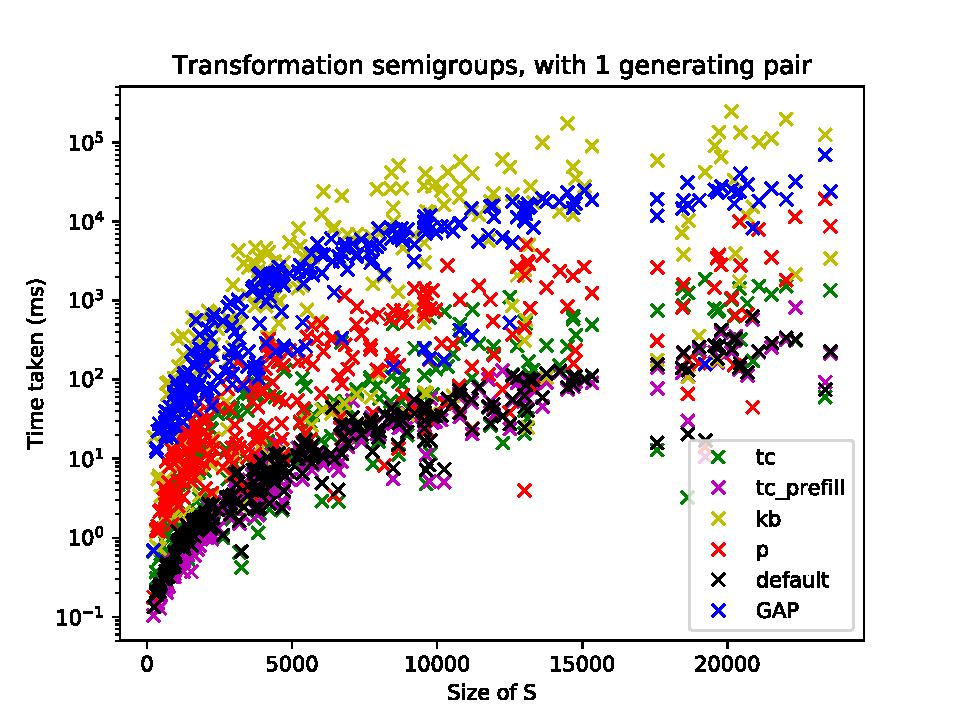
\includegraphics[width=\textwidth]{pics/ch-pairs/bench-trans-1p-times}
  \caption{Performance of the algorithms on 5000 transformation semigroups, with
    one generating pair}
  \label{fig:bench-trans-1p-times}
\end{figure}

\begin{figure}[h]
  \centering
  \includegraphics[width=\textwidth]{pics/ch-pairs/bench-trans-2p-times}
  \caption{Performance of the algorithms on 5000 transformation semigroups, with
    two generating pairs}
  \label{fig:bench-trans-2p-times}
\end{figure}

\begin{figure}[h]
  \centering
  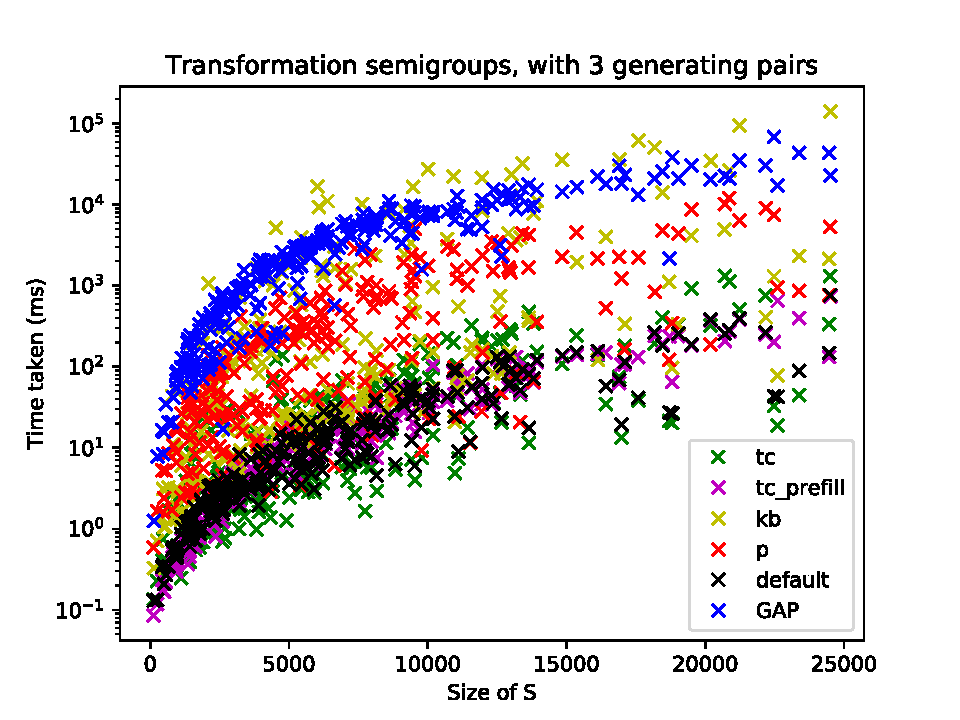
\includegraphics[width=\textwidth]{pics/ch-pairs/bench-trans-3p-times}
  \caption{Performance of the algorithms on 5000 transformation semigroups, with
    three generating pairs}
  \label{fig:bench-trans-3p-times}
\end{figure}

Figure \ref{fig:bench-trans-1p-times} shows the results of a set of 5000 tests
on transformation semigroups.  In each test, $3$ transformations of degree $6$
were chosen at random, and used to generate a semigroup $S$ (any semigroup of
size over $10000$ was rejected).  The elements of $S$ were computed, and a pair
of elements was chosen at random to generate a congruence $\rho$.  Three more
pairs were chosen at random, and each of the different algorithms described in
this chapter was used to determine whether each pair was contained in $\rho$.
Similar tests were also conducted using $2$ and $3$ generating pairs for $\rho$,
as shown in \ref{fig:bench-trans-2p-times} and \ref{fig:bench-trans-3p-times}.
The time taken to return an answer was recorded in each case, and these figures
were compared to one another.  The algorithms used were:
\begin{itemize}
\item Todd-Coxeter (\texttt{tc}),
\item Todd-Coxeter with pre-filled table (\texttt{tc\_prefill}),
\item Knuth-Bendix (\texttt{kb}),
\item pair orbit enumeration (\texttt{p}),
\item the parallel method described in this chapter (\texttt{default}),
\item and the method implemented in the library of GAP (\texttt{GAP}).
\end{itemize}

As can be seen in Figure \ref{fig:bench-trans-1p-times}, the pre-filled Todd-Coxeter
method is the most likely to complete fastest, with regular Todd-Coxeter winning
in a sizeable minority of cases.  This backs up the anecdotal observations group
theorists have made \cite{havascomparing} that Todd-Coxeter tends to perform
faster than Knuth-Bendix.  We may also observe that pair orbit enumeration
sometimes completes almost instantly, which makes some sense when we consider
how little work the algorithm does when there are very few non-reflexive pairs
in the congruence.  The Knuth-Bendix procedure lags behind badly on these
examples, taking even longer than the built-in methods in GAP.  These results
are a justification for the decision to run only the Todd-Coxeter algorithms in
the case of a finite, concrete semigroup.

Figures \ref{fig:bench-trans-2p-times} and \ref{fig:bench-trans-3p-times} show
that with a higher number of generating pairs, the pair orbit enumeration
algorithm suffers badly---this can be understood, since it generally has to
enumerate more pairs when the generating set is larger.  However, with more
generating pairs \texttt{tc} tends to perform relatively better, since there are
likely to be fewer congruence classes and therefore fewer rows in the coset
table.

\begin{figure}[h]
  \centering
  \includegraphics[width=\textwidth]{pics/ch-pairs/bench-trans-1p-tccomp}
  \caption{Comparison between the two Todd-Coxeter methods, for transformation
    semigroups with one generating pair}
  \label{fig:bench-trans-1p-tccomp}
\end{figure}

\begin{figure}[h]
  \centering
  \includegraphics[width=\textwidth]{pics/ch-pairs/bench-trans-2p-tccomp}
  \caption{Comparison between the two Todd-Coxeter methods, for transformation
    semigroups with two generating pairs}
  \label{fig:bench-trans-2p-tccomp}
\end{figure}

\begin{figure}[h]
  \centering
  \includegraphics[width=\textwidth]{pics/ch-pairs/bench-trans-3p-tccomp}
  \caption{Comparison between the two Todd-Coxeter methods, for transformation
    semigroups with three generating pairs}
  \label{fig:bench-trans-3p-tccomp}
\end{figure}

This tendency is illustrated further in Figures \ref{fig:bench-trans-1p-tccomp},
\ref{fig:bench-trans-2p-tccomp} and \ref{fig:bench-trans-3p-tccomp}, which
compare the standard Todd-Coxeter algorithm with the pre-filled version, arranged
according to whether the congruence in question has many or few classes relative
to its size.  The $x$ axis in these figures is
$$(\text{Number of congruence classes} - 1) / (\text{Size of~} S - 1),$$
a scale from $0$ to $1$, where $0$ represents a universal congruence and $1$
represents a trivial congruence.  Since the size of $S$ is a major factor in how
long any algorithm takes to run, only the ratio of \texttt{tc} to
\texttt{tc\_prefill} is shown: a black line is drawn on the graphs to indicate
the length of time taken by \texttt{tc\_prefill}, and a data point is then
plotted for each test, showing how many times as long \texttt{tc} took to
complete.  As can be seen, \texttt{tc} often wins when there are relatively few
large classes, and \texttt{tc\_prefill} is much more likely to win when there are
many small classes.  This reinforces the idea given in Examples \ref{ex:good-tc}
and \ref{ex:good-tc-prefill}, that the winning algorithm may depend on number of
classes, and it is therefore not clear in advance which algorithm may be better.

\begin{figure}[h]
  \centering
  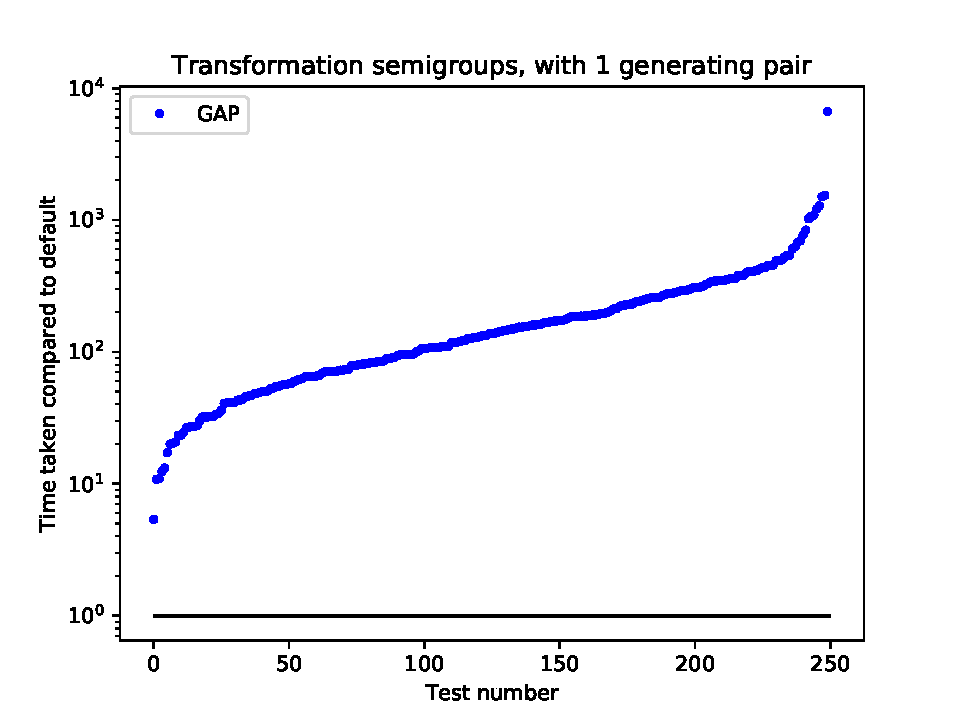
\includegraphics[width=\textwidth]{pics/ch-pairs/bench-trans-1p-gap}
  \caption{Comparison between \texttt{libsemigroups} and the GAP library, for
    transformation semigroups with one generating pair}
  \label{fig:bench-trans-1p-gap}
\end{figure}

\begin{figure}[h]
  \centering
  \includegraphics[width=\textwidth]{pics/ch-pairs/bench-trans-2p-gap}
  \caption{Comparison between \texttt{libsemigroups} and the GAP library, for
    transformation semigroups with two generating pairs}
  \label{fig:bench-trans-2p-gap}
\end{figure}

\begin{figure}[h]
  \centering
  \includegraphics[width=\textwidth]{pics/ch-pairs/bench-trans-3p-gap}
  \caption{Comparison between \texttt{libsemigroups} and the GAP library, for
    transformation semigroups with three generating pairs}
  \label{fig:bench-trans-3p-gap}
\end{figure}

Figures \ref{fig:bench-trans-1p-gap}, \ref{fig:bench-trans-2p-gap} and
\ref{fig:bench-trans-3p-gap} show data from the same tests, plotted not by
the size of the semigroup, but simply in order of the ratio between GAP's
runtime and that of the default method in \texttt{libsemigroups}.  As can be
seen, the \texttt{libsemigroups} methods run much faster than the GAP methods in
almost all cases, with the GAP methods taking as much as $2800$ times as long
for one generating pair.  Out of $5000$ tests, GAP performed better in only $12$
cases, and these were all tests in which both methods completed in less than
$0.3$ milliseconds.  On tests with two and three generating pairs, GAP was
slower every time.

Further tests were carried out in a similar way, but using finitely presented
semigroups instead of concrete semigroups.  The main difference between these
tests and the ones described previously is that for each transformation
semigroup $S$ which was generated, a finite presentation $\pres X R$ was found
for $S$, and that presentation was used in tests instead of the concrete
semigroup $S$ itself.  This is intended to test which algorithms are effective
when the elements of the semigroup are not known in advance.

In order to produce a further comparison, the tests for finitely presented
semigroups were also run with the \textit{kbmag} package for GAP \cite{kbmag}.
The results are shown on the graphs with the name \texttt{kbmag}.

\begin{figure}[h]
  \centering
  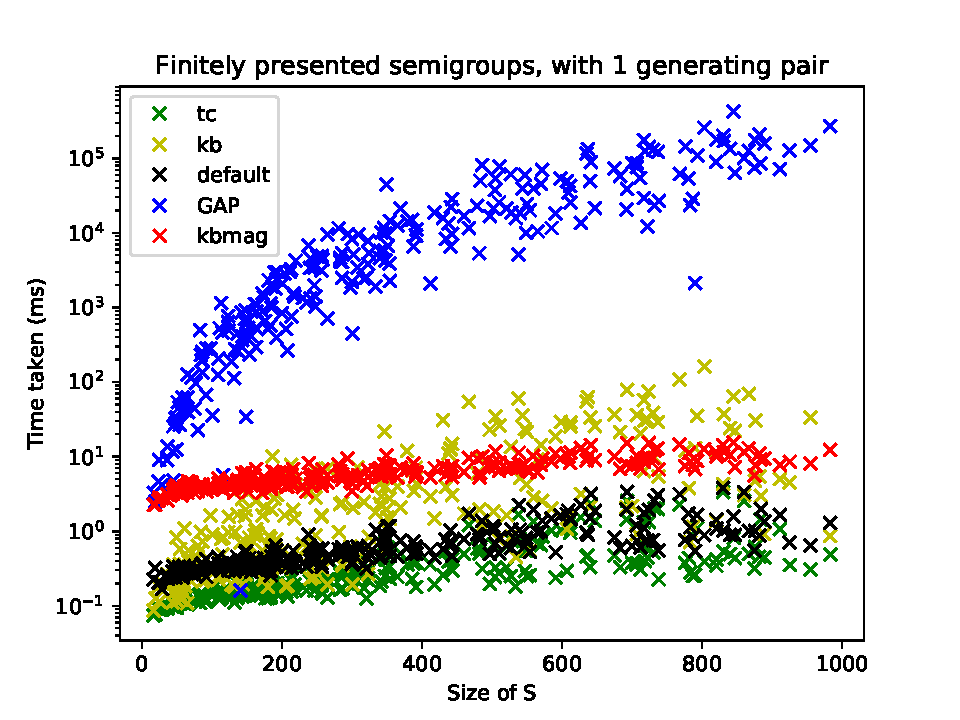
\includegraphics[width=\textwidth]{pics/ch-pairs/bench-fp-1p-times}
  \caption{Performance of the algorithms on $1000$ finitely presented semigroups
    with one generating pair}
  \label{fig:bench-fp-1p-times}
\end{figure}

\begin{figure}[h]
  \centering
  \includegraphics[width=\textwidth]{pics/ch-pairs/bench-fp-2p-times}
  \caption{Performance of the algorithms on $1000$ finitely presented semigroups
    with two generating pairs}
  \label{fig:bench-fp-2p-times}
\end{figure}

\begin{figure}[h]
  \centering
  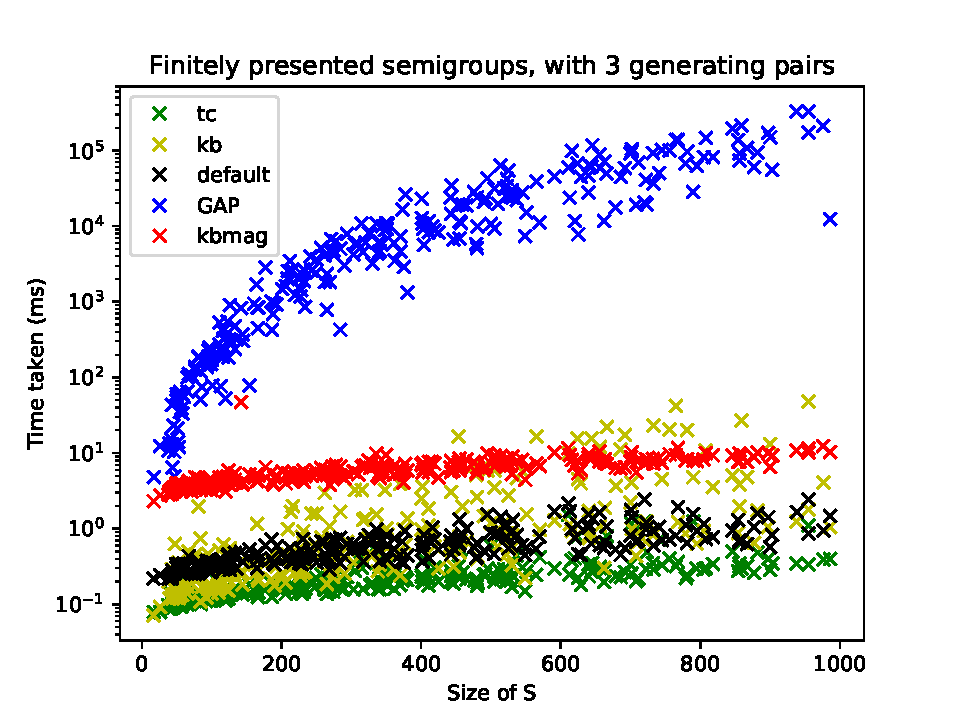
\includegraphics[width=\textwidth]{pics/ch-pairs/bench-fp-3p-times}
  \caption{Performance of the algorithms on $1000$ finitely presented semigroups
    with three generating pairs}
  \label{fig:bench-fp-3p-times}
\end{figure}

\begin{figure}[h]
  \centering
  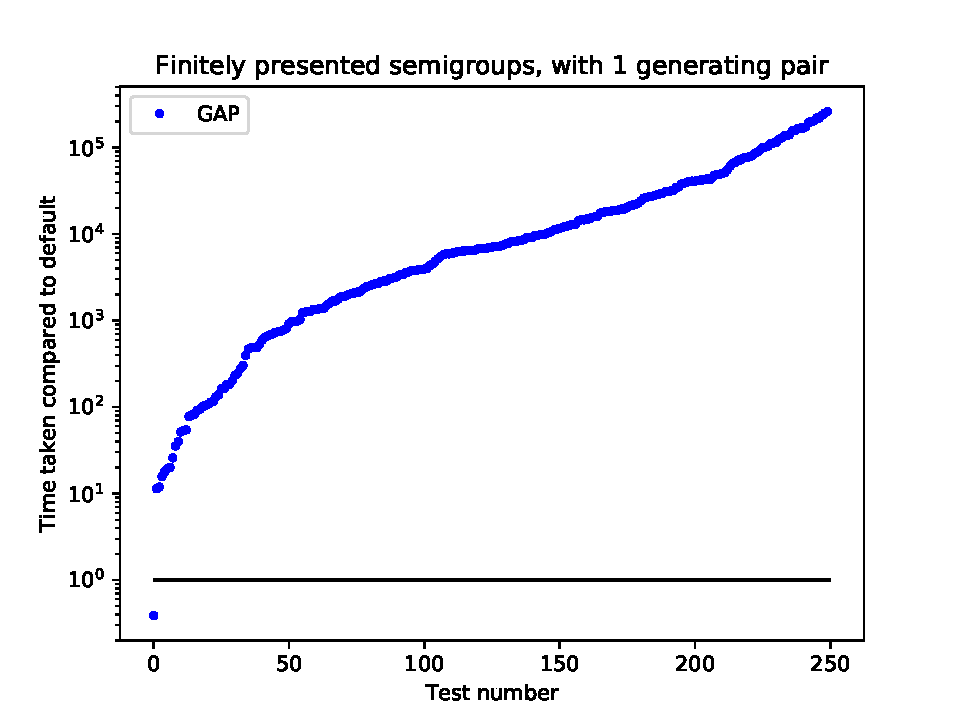
\includegraphics[width=\textwidth]{pics/ch-pairs/bench-fp-1p-gap}
  \caption{Comparison between \texttt{libsemigroups} and the GAP library, for
    finitely presented semigroups and one generating pair}
  \label{fig:bench-fp-1p-gap}
\end{figure}

\begin{figure}[h]
  \centering
  \includegraphics[width=\textwidth]{pics/ch-pairs/bench-fp-2p-gap}
  \caption{Comparison between \texttt{libsemigroups} and the GAP library, for
    finitely presented semigroups and two generating pairs}
  \label{fig:bench-fp-2p-gap}
\end{figure}

\begin{figure}[h]
  \centering
  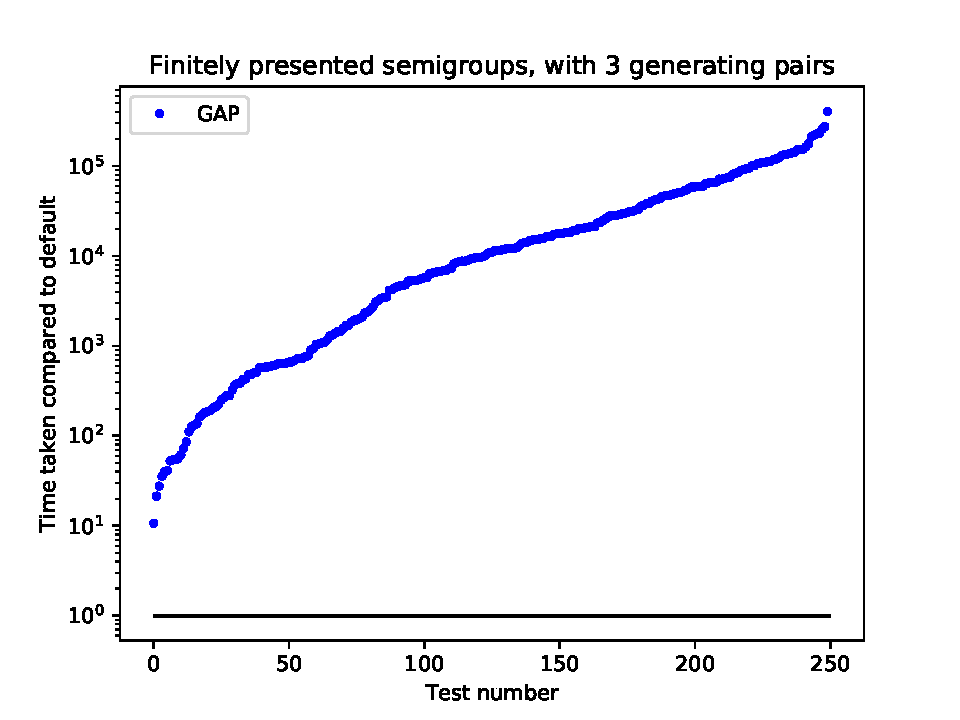
\includegraphics[width=\textwidth]{pics/ch-pairs/bench-fp-3p-gap}
  \caption{Comparison between \texttt{libsemigroups} and the GAP library, for
    finitely presented semigroups and three generating pairs}
  \label{fig:bench-fp-3p-gap}
\end{figure}

As can be seen in Figures \ref{fig:bench-fp-1p-gap} to \ref{fig:bench-fp-3p-gap}, the
performance of the GAP library over finitely presented semigroups is far worse
than it was for concrete semigroups, taking as much as $400,000$ times as long
as \texttt{libsemigroups} to complete.  Due to the excessive times GAP took to
complete some tests, the size of semigroups was restricted to $1000$, and only
$1000$ tests were carried out.  In these tests, unlike for concrete semigroups,
Knuth-Bendix tended to outperform GAP, but in
general Todd-Coxeter methods were still faster.  It should be noted, however,
that these were all congruences that were guaranteed in advance to have a finite
number of classes.  An arbitrary congruence on a finitely presented semigroup
may have an infinite number of classes, and there are many examples in which
Knuth-Bendix can return an answer but Todd-Coxeter cannot (see Example
\ref{ex:good-kbfp}).

\textit{kbmag} generally performed worse in tests than Todd-Coxeter, but was
comparable to our implementation of Knuth-Bendix (TODO: our KB will probably
improve a lot soon).  It generally took around $10$ times as long as the
complete parallel method (\texttt{default} on the graphs).

\section{Future work}

The parallel approach described in this chapter is quite open-ended, and could
be extended or improved in several ways.  Given more time to spend on the
project, these are areas which could bear investigation.

\subsection{Pre-filling Todd-Coxeter with a left Cayley graph}
\label{sec:prefill-left}
The pre-filled Todd-Coxeter algorithm, as described in Section
\ref{sec:tc-prefill}, works by starting the procedure with a right Cayley graph
for $S$.  In \texttt{libsemigroups} and in the Semigroups package for GAP, a
right Cayley graph for a semigroup is found using the Froidure-Pin method, which
also returns the corresponding left Cayley graph.  Hence, we may also wish to
find a way to use the left Cayley graph in the pre-filling process.

As mentioned in Section \ref{sec:tc-l-r}, it is possible to use Todd-Coxeter
with a reversed multiplication, essentially studying a semigroup anti-isomorphic
to $S$.  It would be possible to apply the same principle, reverse the
multiplication of elements in $S$, and thus use the left Cayley graph instead of
the right Cayley graph in pre-filling.  This could be run as an additional
thread in the parallel procedure.

In many cases, using the left Cayley graph might be very similar in terms of
performance to using the right.  However, some semigroups have left and right
Cayley graphs which are very different.  Consider, for example, the right zero
semigroup $\RZ_n$, which has $n$ generators, $n$ elements, and the
multiplication $xy=y$ for any $x,y \in \RZ_n$.  Its right Cayley graph is the
complete digraph, where any element can be mapped to any other element using the
appropriate generator.  Its left Cayley graph is totally disconnected, with each
vertex $v$ in a single trivial connected component with $n$ edges taking $v$ to
$v$.  With such different left and right Cayley graphs, it seems likely that one
piece of information would be much more helpful than the other in calculating
congruences on the semigroup.

\subsection{Interaction between Knuth-Bendix and Todd-Coxeter}
\label{sec:linking-kb-tc}
The Knuth-Bendix and Todd-Coxeter algorithms, as described in this chapter, do
not interact with each other in any way.  The Knuth-Bendix process runs in one
thread, and the Todd-Coxeter process runs in another.  However, information from
one could perhaps be shared with the other.

The main objective of Knuth-Bendix is the addition of new rewriting rules to a
rewriting system $\rws$ to satisfy the condition of confluence: if a critical
pair is found, and a new rule $u \to v$ is added to $\rws$, then this gives us a
pair of words $(u,v)$ which represents a pair of congruent elements in the congruence we
are studying.  If a Todd-Coxeter procedure is running in parallel, it would be
possible to send the pair of words $(u,v)$ to the Todd-Coxeter thread, which
at its next convenience would run \textsc{Coinc(Trace($1, u$), Trace($1, v$))}
to identify the two corresponding rows in the table.

Conversely, Todd-Coxeter may find information which could be used by
Knuth-Bendix.  Firstly, it is trivial to record, for each row $i$ of the table,
the word $w_i$ which was first used to describe it: row $1$ is identified with
the empty word ($w_1 := \varepsilon$), and if a row is created using
\textsc{Add($i, x$)} then it is assigned the word $w_ix$.  For each row $i$, we
now have \textsc{Trace}$(1, w_i) = i$; that is, each row has a word which can
act as a representative for its congruence class.

If, in a normal run of Todd-Coxeter, it is found that two rows $i$ and $j$
represent the same class and must be combined, then this immediately gives a
pair of words $(w_i,w_j)$ which represent the same congruence class.  This pair
of words can be sent to a parallel instance of Knuth-Bendix, which can add it as
a rule $w_i \to w_j$ (or $w_j \to w_i$, as dictated by the chosen ordering).

It may be that this sharing of knowledge between the two algorithms would
greatly increase the speed of certain calculations; or it may be that the time
and space overhead required to implement these ideas would be so great that the
algorithms would not speed up at all.  Experiments with this idea might show it
to be useful, or might suggest that it is not worth pursuing.

\subsection{Using concrete elements in Todd-Coxeter}
\label{sec:tc-concrete-elms}
The Todd-Coxeter procedure uses a finite presentation $\pres X R$ and a set of
extra pairs $\mathbf{W}$ in order to calculate information about a congruence
over a semigroup $S$.  If $S$ is a concrete semigroup, then $\pres X R$ and $W$
must be calculated before the beginning of Todd-Coxeter, so that the procedure
can use them as parameters.  However, once this information has been calculated,
no other information about $S$ is used for the rest of the algorithm, which only
deals with words, abstract generators and relations.

It may prove helpful to use the concrete elements from $S$ in the Todd-Coxeter
procedure, if they are known.  For instance, when \textsc{Add($i, x$)} for some
row $i$ and generator $x$, it would be possible to find an element corresponding
to row $i$, find the element corresponding to the generator $x$, multiply the
two, and see whether a row already exists which represents that element.  In
this way, we can avoid the unnecessary creation of new rows which would only be
deleted by \textsc{Coinc} later.

The pre-filling of Todd-Coxeter tables is one use of the concrete elements that
we have already described and implemented, but they may be many more which would
be effective.

\subsection{Left and right congruences with Knuth-Bendix}
\label{sec:kb-l-r}
The parallel method in this chapter, and its implementation in
\texttt{libsemigroups}, include support for left congruences and right
congruences, as well as the more important two-sided congruences.  Currently,
Todd-Coxeter and pair enumeration are the only methods which support left and
right congruences, while Knuth-Bendix is only applied in the two-sided case.
However, there does exist a variation of the Knuth-Bendix procedure which could
compute left and right congruences in some limited cases, namely when the
semigroup in question is the free monoid $X^*$ for some set $X$.  The procedure
involves appending an extra generator $\#$ and adding it as a prefix to all the
words in the set of generating pairs $W$.  It is described in more detail in
\cite[\S 2.8]{sims}.

Since this is limited to left and right congruences over free monoids, it is
limited in its possible use for the algorithm described in this chapter.
However, it might cause a performance improvement in those few cases.

% TODO: In the GAP library, anything interesting they might do

\clearpage

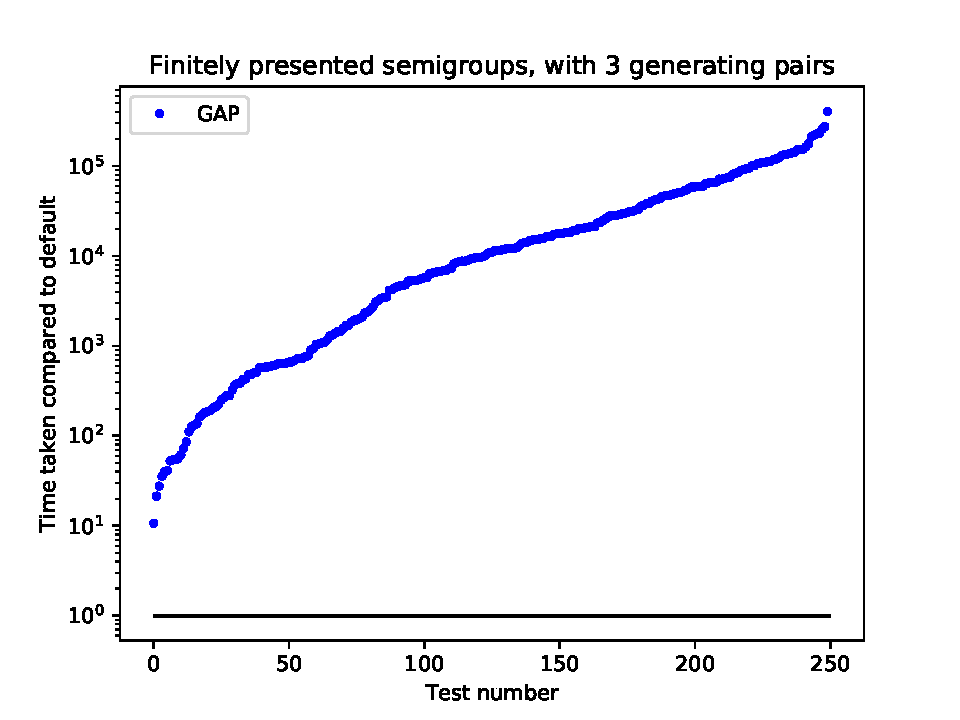
\includegraphics[width=\textwidth]{pics/ch-pairs/bench-fp-3p-gap}
\includegraphics[width=\textwidth]{pics/ch-pairs/bench-fp-1p-bynrclasses}
\includegraphics[width=\textwidth]{pics/ch-pairs/bench-fp-2p-bynrclasses}
\includegraphics[width=\textwidth]{pics/ch-pairs/bench-fp-3p-bynrclasses}
\includegraphics[width=\textwidth]{pics/ch-pairs/bench-fp-vp-bynrclasses}
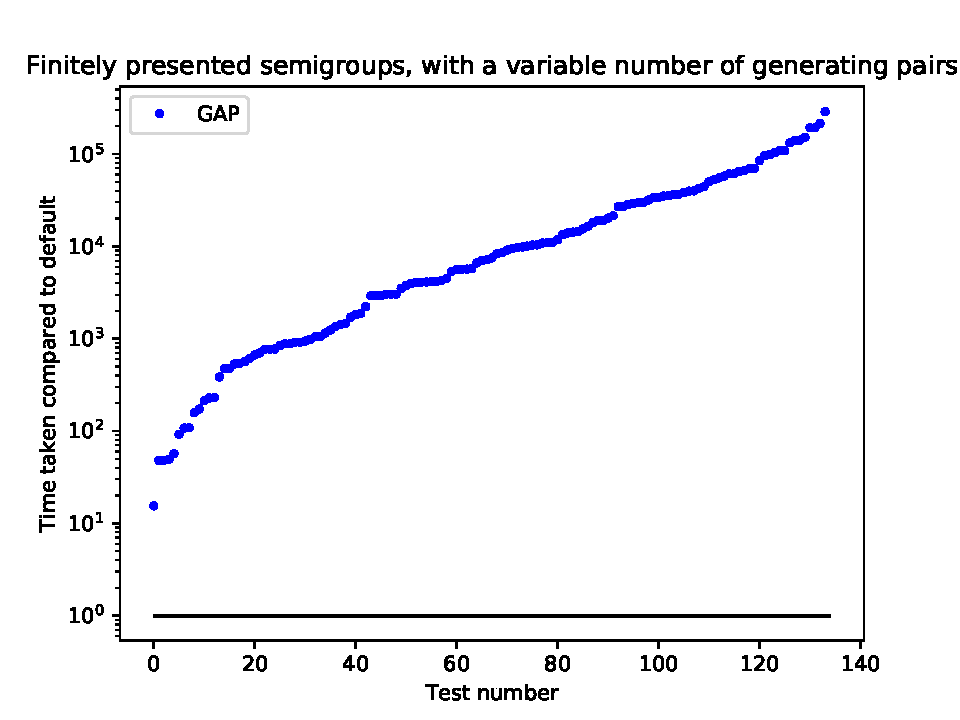
\includegraphics[width=\textwidth]{pics/ch-pairs/bench-fp-vp-gap}
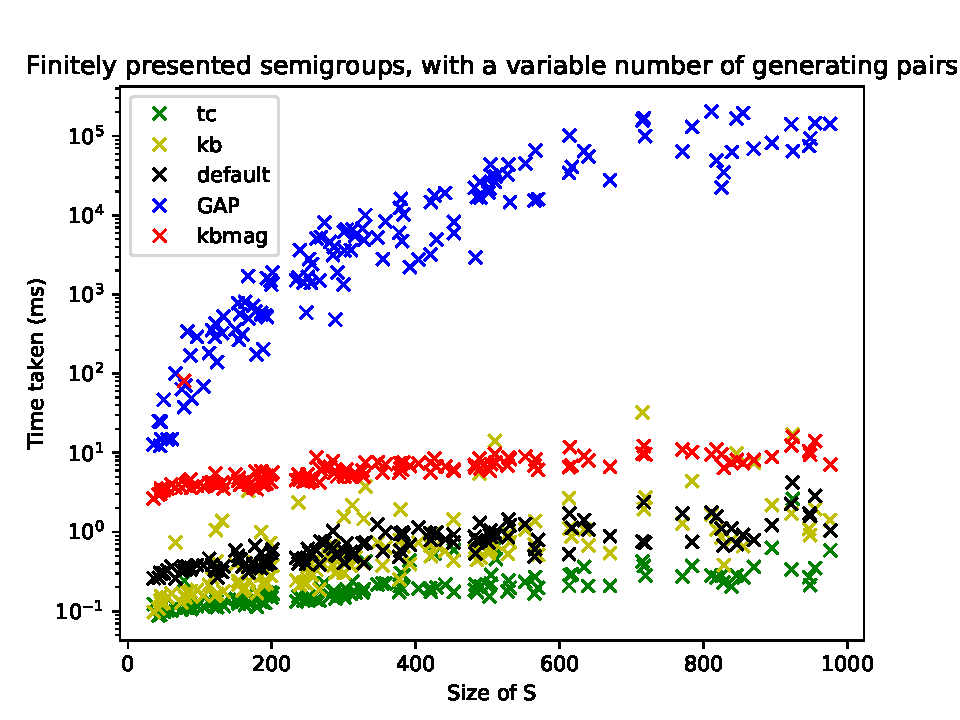
\includegraphics[width=\textwidth]{pics/ch-pairs/bench-fp-vp-times}
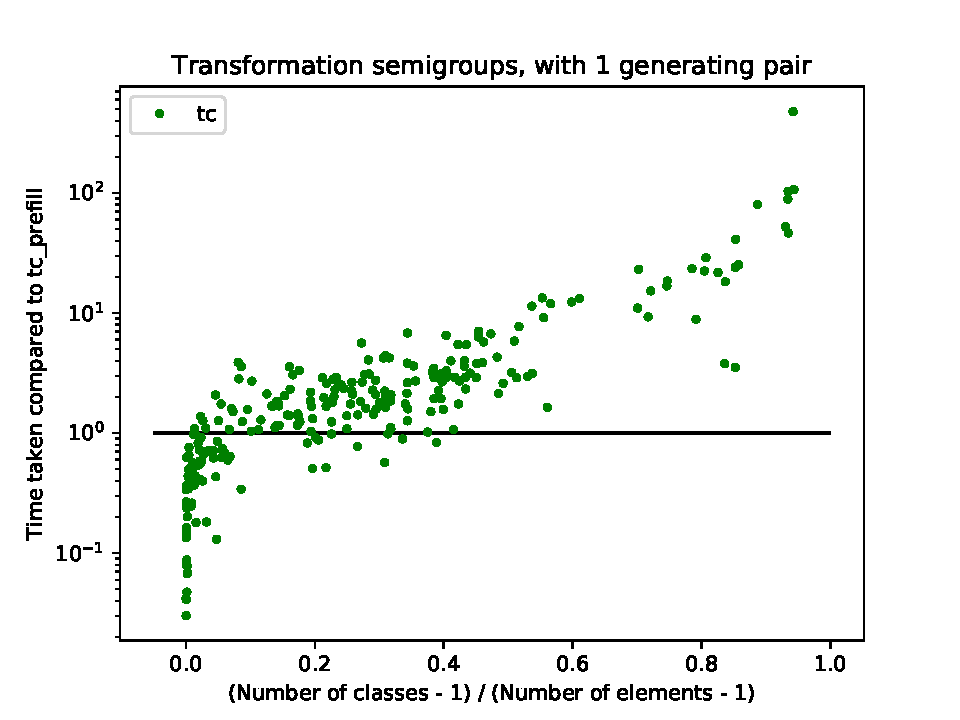
\includegraphics[width=\textwidth]{pics/ch-pairs/bench-trans-tc-1p-tccomp}
\includegraphics[width=\textwidth]{pics/ch-pairs/bench-trans-tc-1p-times}
\includegraphics[width=\textwidth]{pics/ch-pairs/bench-trans-tc-2p-tccomp}
\includegraphics[width=\textwidth]{pics/ch-pairs/bench-trans-tc-2p-times}
\includegraphics[width=\textwidth]{pics/ch-pairs/bench-trans-tc-3p-tccomp}
\includegraphics[width=\textwidth]{pics/ch-pairs/bench-trans-tc-3p-times}
\includegraphics[width=\textwidth]{pics/ch-pairs/bench-trans-vp-bynrclasses}
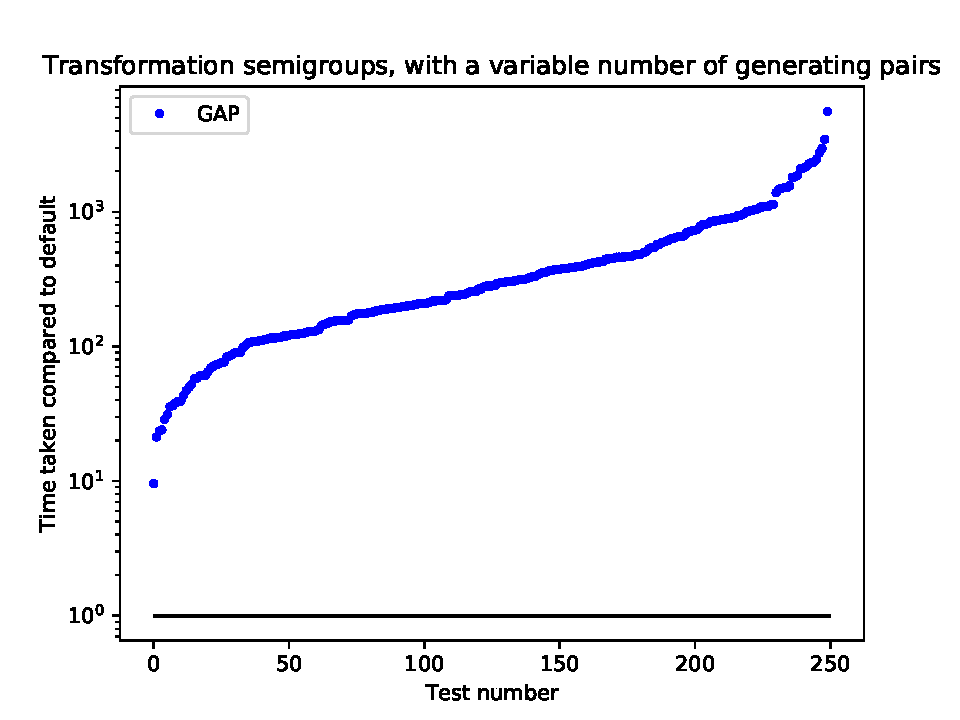
\includegraphics[width=\textwidth]{pics/ch-pairs/bench-trans-vp-gap}
\includegraphics[width=\textwidth]{pics/ch-pairs/bench-trans-vp-tccomp}
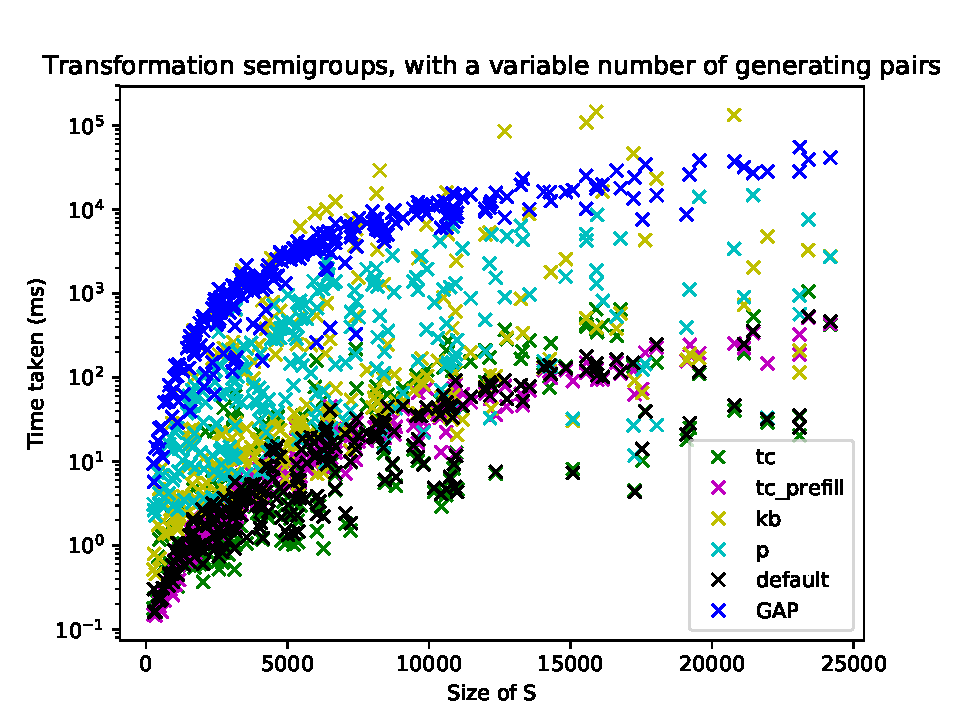
\includegraphics[width=\textwidth]{pics/ch-pairs/bench-trans-vp-times}

\clearpage

\includegraphics[width=\textwidth]{pics/ch-pairs/bench-fp-vp-right-gap}
\includegraphics[width=\textwidth]{pics/ch-pairs/bench-fp-vp-right-times}
